%\documentclass[pfe]{./tpl/isipfe}
\documentclass[12pt]{tpl/isipfe}
\graphicspath{{./img/}}

%\usepackage{hyperref}
\usepackage{enumitem}

\newenvironment{changemargin}[2]{%
\begin{list}{}{%
\setlength{\leftmargin}{#1}%
\setlength{\rightmargin}{#2}%
}%
\item[]}
{\end{list}}

\makeatletter

%================= front cover variables =================%

\newcommand{\secondAuthor}[1]{\gdef\@secondAuthor{#1}}%
\newcommand{\@secondAuthor}{\@latex@warning@no@line{No \noexpand\secondAuthor given}}

\newcommand{\diplomaName}[1]{\gdef\@diplomaName{#1}}%
\newcommand{\@diplomaName}{\@latex@warning@no@line{No \noexpand\diplomaName given}}

\newcommand{\speciality}[1]{\gdef\@speciality{#1}}%
\newcommand{\@speciality}{\@latex@warning@no@line{No \noexpand\speciality given}}

\newcommand{\proFramerName}[1]{\gdef\@proFramerName{#1}}%
\newcommand{\@proFramerName}{\@latex@warning@no@line{No \noexpand\proFramerName given}}

\newcommand{\proFramerSpeciality}[1]{\gdef\@proFramerSpeciality{#1}}%
\newcommand{\@proFramerSpeciality}{\@latex@warning@no@line{No \noexpand\proFramerSpeciality given}}

\newcommand{\academicFramerName}[1]{\gdef\@academicFramerName{#1}}%
\newcommand{\@academicFramerName}{\@latex@warning@no@line{No \noexpand\academicFramerName given}}

\newcommand{\academicFramerSpeciality}[1]{\gdef\@academicFramerSpeciality{#1}}%
\newcommand{\@academicFramerSpeciality}{\@latex@warning@no@line{No \noexpand\academicFramerSpeciality given}}

\newcommand{\collegeYear}[1]{\gdef\@collegeYear{#1}}%
\newcommand{\@collegeYear}{\@latex@warning@no@line{No \noexpand\collegeYear given}}

\newcommand{\companyName}[1]{\gdef\@companyName{#1}}%
\newcommand{\@companyName}{\@latex@warning@no@line{No \noexpand\companyName given}}

%================== Signatures variables ==================%

\newcommand{\proSignSentence}[1]{\gdef\@proSignSentence{#1}}%
\newcommand{\@proSignSentence}{\@latex@warning@no@line{No \noexpand\proSignSentence given}}

\newcommand{\academicSignSentence}[1]{\gdef\@academicSignSentence{#1}}%
\newcommand{\@academicSignSentence}{\@latex@warning@no@line{No \noexpand\academicSignSentence given}}

%================== Backcover variables ==================%

\newcommand{\arabicAbstract}[1]{\gdef\@arabicAbstract{#1}}%
\newcommand{\@arabicAbstract}{\@latex@warning@no@line{No \noexpand\arabicAbstract given}}

\newcommand{\arabicAbstractKeywords}[1]{\gdef\@arabicAbstractKeywords{#1}}%
\newcommand{\@arabicAbstractKeywords}{\@latex@warning@no@line{No \noexpand\arabicAbstractKeywords given}}

\newcommand{\frenchAbstract}[1]{\gdef\@frenchAbstract{#1}}%
\newcommand{\@frenchAbstract}{\@latex@warning@no@line{No \noexpand\frenchAbstract given}}

\newcommand{\frenchAbstractKeywords}[1]{\gdef\@frenchAbstractKeywords{#1}}%
\newcommand{\@frenchAbstractKeywords}{\@latex@warning@no@line{No \noexpand\frenchAbstractKeywords given}}

\newcommand{\englishAbstract}[1]{\gdef\@englishAbstract{#1}}%
\newcommand{\@englishAbstract}{\@latex@warning@no@line{No \noexpand\englishAbstract given}}

\newcommand{\englishAbstractKeywords}[1]{\gdef\@englishAbstractKeywords{#1}}%
\newcommand{\@englishAbstractKeywords}{\@latex@warning@no@line{No \noexpand\englishAbstractKeywords given}}

\newcommand{\companyEmail}[1]{\gdef\@companyEmail{#1}}%
\newcommand{\@companyEmail}{\@latex@warning@no@line{No \noexpand\companyEmail given}}

\newcommand{\companyTel}[1]{\gdef\@companyTel{#1}}%
\newcommand{\@companyTel}{\@latex@warning@no@line{No \noexpand\companyTel given}}

\newcommand{\companyFax}[1]{\gdef\@companyFax{#1}}%
\newcommand{\@companyFax}{\@latex@warning@no@line{No \noexpand\companyFax given}}

\newcommand{\companyAddressFR}[1]{\gdef\@companyAddressFR{#1}}%
\newcommand{\@companyAddressFR}{\@latex@warning@no@line{No \noexpand\companyAddressFR given}}

\newcommand{\companyAddressAR}[1]{\gdef\@companyAddressAR{#1}}%
\newcommand{\@companyAddressAR}{\@latex@warning@no@line{No \noexpand\companyAddressAR given}}

%============= cmd for inserting blank page =============%
\newcommand\blankpage{%
    \null
    \thispagestyle{empty}%
    \addtocounter{page}{-1}%
    \newpage}

%================ document main language ================%
%\selectlanguage{english}
\selectlanguage{french}

%================== required packages ===================%

\usepackage{tcolorbox}
\usepackage{afterpage}
\usepackage{array,longtable,multirow}% http://ctan.org/pkg/{array,longtable,multirow}
\usepackage{pifont}

\usepackage{pdflscape}
\usepackage{rotating}
\usepackage{wrapfig}

%================== chapter numbering ===================%
\renewcommand{\thesection}{\Roman{section}}
\renewcommand{\thesubsection}{\thesection.\arabic{subsection}}
\renewcommand{\thesubsubsection}{\thesubsection.\arabic{subsubsection}}

\usepackage{titlesec}
\usepackage{titletoc}
\usepackage{appendix}
\usepackage{hyperref}

\makeatletter
    
\titlecontents{chapter}%
    [0em]% 
    {\addvspace{2em}}%
    {\bfseries\@chapapp\ \thecontentslabel:\quad}% 
    {\hspace{-0em}}% 
    {\hfill\contentspage}% 
    [\addvspace{0pt}]% 
    
% the command `\makeindex` is mandatory to create the index file main.idx
% https://tex.stackexchange.com/questions/9913/input-index-file-not-found
\makeindex

\begin{document}
    
%=========== You MUST type your information here ==========%
% global_config.tex file is designed to configure your     %
% cover pages (main, back and black covers)                %
%==========================================================%

%============= Config new columns type ==============%
\newcolumntype{L}{>{\raggedright\arraybackslash}}
\newcolumntype{R}{>{\raggedleft\arraybackslash}}
\newcolumntype{C}{>{\centering\arraybackslash}}
%==================================================%

%========= Config the cover section ==========%

\title{REFONTE DU MODULE DE GESTION DES CANDIDATS: DE L'OUTIL BYBLOS VERS UNE ARCHITECTURE MICROSERVICES}

\author{Mohamed Amine Ayed}
%%% if necessary
% Set isBinomal to true and type second author name
%\setboolean{isBinomal}{true}
%\secondAuthor{Prénom NOM}

\diplomaName{Diplôme National d'Ingénieur en Sciences Appliquées et Technologiques}
\speciality{Génie Logiciel et Système d'Informations}
%\speciality{Génie des Télécommunications et Réseaux}
%\speciality{Génie Informatique des Systèmes Industriels}

%% Encadrant professionnel
\proFramerName{Madame Mariem Chater}
\proFramerSpeciality{Scrum Master}
%\proFramerName{Monsieur DRIDI Foued}
%\proFramerSpeciality{Ingénieur Sécurité}

%% Encadrant académique
\academicFramerName{Madame Asma Mabrouk}
\academicFramerSpeciality{Maître Assistant(e)}

%% Entreprise d'accueil
\companyName{Talan Tunisie Consulting}

%% Année universitaire
\collegeYear{2019 - 2020}

%%%%%% Signatures section %%%%%%

% You can simply remove theses sentences by typing an empty string
% \proSignSentence{}

\proSignSentence{J'autorise l'étudiant à faire le dépôt de son rapport de stage en vue d'une soutenance.}

\academicSignSentence{J'autorise l'étudiant à faire le dépôt de son rapport de stage en vue d'une soutenance.}

%% To use latin characters inside the arabic text
% just put them inside the command \textLR{}
%%%%

%%% FR
\frenchAbstract{Le présent rapport synthétise le travail effectué dans le cadre du projet de fin d’études pour l’obtention du diplôme national d’ingénieur en informatique au sein de l’entreprise Talan Tunisie Consulting. Le travail consiste à une refonte du module de gestion des candidats de BYBLOS qui est un ERP(Entretprise Ressource Planning) de Talan Tunisie Consulting, en se basant sur une architecture en microservices ainsi que trouver des alternatifs pour quelques technologies qui ont présenté leurs limites.}

\frenchAbstractKeywords{Microservices, Spring Boot, Spring Cloud, Spring Data, QueryDsl, Angular}

%%% EN
\englishAbstract{
This report summarizes the work carried out as part of the end-of-study project for obtaining the national software engineering degree within the company Talan Tunisia Consulting. The work consists in redesigning the BYBLOS candidate management module, which is an ERP (Enterprise Resource Planning) of Talan Tunisia Consulting, based on a microservices architecture and finding alternatives for some technologies that have presented their limitations.}

\englishAbstractKeywords{Microservices, Spring Boot, Spring Cloud, Spring Data, QueryDsl, Angular}

%% if you want to get rid of the company address just set the boolean variable to false
% PS : it's optional
\setboolean{wantToTypeCompanyAddress}{false}

\companyEmail{contact@company.com}
\companyTel{71 111 111}
\companyFax{71 222 222}
\companyAddressFR{Rue du Lac de Constance, Tunis}
    
    \frontmatter
        
%== It's advised to not modify the content of this file ===%
% To set your information, go to global_config.tex file    %
%==========================================================%

\thispagestyle{cover}%
\newgeometry{bottom=25mm,left=20mm,top=15mm,right=20mm}
\hspace{-47pt}
\begin{minipage}[l]{0.2\columnwidth}
\vspace{6mm}

\includegraphics[width=1.1\columnwidth]{img/tekup.png}\\
\end{minipage}
\hfill
\begin{minipage}[l]{0.6\columnwidth}
\centering
\footnotesize
\textbf{{République Tunisienne}}\\
\vspace{1.5mm}
\textbf{{Ministère de l'Enseignement Supérieur\\
et de la Recherche Scientifique}}\\
\vspace{1.5mm}
%\textbf{{Université de Tunis El Manar}}\\
\vspace{1.5mm}
\textbf{{École Supérieur Privée d'ingénierie et de technologie}}\\
\vspace{1.5mm}
\textbf{{TEK-UP}}\\
\vspace{1.5mm}
\end{minipage}
\hfill
\begin{minipage}[l]{0.02\columnwidth}
\end{minipage}
\hfill
\begin{minipage}[l]{0.2\columnwidth}
\vspace{6mm}

\includegraphics[width=1.1\columnwidth]{img/talan.png}\\
\end{minipage}
\vskip1.5cm

\begin{center}
{\LARGE{\textbf{\textsc{Rapport de Projet de Fin d'Études}}}}\\
\vskip0.5cm
\large

{\textbf{Présenté en vue de l'obtention du}}\\
\vskip2mm
{\textbf{\@diplomaName}}\\
{\textbf{Spécialité : \@speciality}}\\
{}
\end{center}

\begin{center}
\textrm{Réalisé par}\\
\vskip0.3cm
{\ifthenelse{\boolean{isBinomal}}
    {% IF TRUE
        \begin{center}
            \large\textbf{\@author}~~~~~ et ~~~~~
            \large\textbf{\@secondAuthor}
        \end{center}
    }
    {\Large\textbf{\@author}}% FALSE
}
\vskip12mm

\definecolor{isiBlue}{RGB}{31, 78, 121}

\begin{changemargin}{-9mm}{0cm}
\begin{minipage}[l]{1.1\columnwidth}
\begin{tcolorbox}[colframe=isiBlue,colback=white,boxrule=0pt,toprule=3pt,bottomrule=3pt,arc=0pt,top=0mm,right=0mm,left=0mm,bottom=0mm,boxsep=0.5mm]{
    \begin{tcolorbox}[colframe=isiBlue,colback=white, boxrule=0pt,toprule=1pt,bottomrule=1pt,arc=0pt,enlarge bottom by=-0.9mm, auto outer arc]
        \centering
        {\huge\textbf{\@title}}
    \end{tcolorbox}
}
\end{tcolorbox}
\end{minipage}
\end{changemargin}

\end{center}
\vskip8mm%

\begin{center}
\large
\begin{minipage}[c]{0.28\columnwidth}
Encadrant professionnel:\\
Encadrant académique:
\end{minipage}
\hfill
\begin{minipage}[c]{0.42\columnwidth}
\textbf{\@proFramerName}\\
\textbf{\@academicFramerName}
\end{minipage}
\hfill
\begin{minipage}[c]{0.26\columnwidth}
\@proFramerSpeciality\\
\@academicFramerSpeciality
\end{minipage}
\end{center}
\vskip16mm

\afterpage{\blankpage}
        \include{tpl/cover_page_black}
        \thispagestyle{empty}

\begin{center}
    \begin{minipage}[l]{1\columnwidth}
        \begin{tcolorbox}[colback=white,boxrule=5pt,arc=10pt,height=105mm]{
            \vspace{2cm}
            \large \@proSignSentence
            \vspace{1mm}
            \begin{center}
                \Large
                Encadrant professionnel, \textbf{\@proFramerName}
            \end{center}
            \vspace{5mm}
            \hspace{0.71\columnwidth}\textbf{\large Signature et cachet}
        }
        \end{tcolorbox}
    \end{minipage}
    
    \vspace{2cm}
    
    \begin{minipage}[l]{1\columnwidth}
        \begin{tcolorbox}[colback=white,boxrule=5pt,arc=10pt,height=105mm]{
            \vspace{2cm}
            \large \@academicSignSentence
            \vspace{1mm}
            \begin{center}
                \Large
                Encadrant académique, \textbf{\@academicFramerName}
            \end{center}
            \vspace{5mm}
            \hspace{0.84\columnwidth}\textbf{\large Signature}
        }
        \end{tcolorbox}
    \end{minipage}
\end{center}
        
        \setcounter{page}{1}
        \chapter*{\Huge Dédicace}
\vspace{8mm}
\vspace{8mm}

\begingroup

\begin{center}
\it \LARGE
    Je dédie ce travail, comme preuve de respect, de gratitude, et de reconnaissance à :\\
    Ma chère famille, pour son affection, sa patience, et ses prières.\\
    Mes meilleurs amis pour leur aide, leur temps, leurs encouragements, leur assistance et leur soutien.\\
    A tous ceux qui ont contribué de près ou de loin à la réalisation de ce travail.
\end{center}



\endgroup

\vspace{8mm}
\begin{flushright}
    \LARGE Toute ma reconnaissance...
\end{flushright}
        \thispagestyle{frontmatter}
        \chapter*{\huge Remerciements}

C’est avec un grand plaisir que je réserve cette page en signe de gratitude et de profonde reconnaissance à tous ceux qui ont bien voulu apporter l’assistance nécessaire au bon déroulement de ce travail.\\
Je remercie tout d'abord \textbf{\@academicFramerName}, maître assistante à TEK-UP, pour son soutien continue et son attention qu'elle n'a cessé de m'apporter tout au long de ce projet en tant qu'encadrante académique. Je tiens à lui exprimer ma gratitude pour apport crucial à ce travail.\\
\\
Ce projet a été effectué au sein de Talan Tunisie. J’adresse mes sincères remerciements à \textbf{Madame Mariem Chater}, le scrum master de l'équipe Byblos, et mon encadrante professionnelle, pou m’avoir aidé à bien mener ce projet, pour son soutien scientifique et sa disponibilité.
\\
\\
Je tiens à remercier également \textbf{Monsieur Hassen Besbes}, Ingénieur senior en java, et mon encadrant technique, lors de ce projet, pour m'aider aux lacunes et aux difficultés techniques et aussi à l'esprit logique de savoir-faire à la face des tâches.
\\
\\
Merci aussi à mes amis qui se reconnaîtront ici, merci pour les moments d’amitié que nous avons partagés. Vous avez toujours été présents pendant les moments les plus difficiles de ma vie professionnelle, j’ai eu beaucoup de chance de vous avoir comme amis.
    
    %Je suis reconnaissant
    
    %J'exprime ma gratitude
    %\large \raggedright Je dédie ce travail à :
    %\vspace{4mm}
    
    %\textbf{\@proFramerName},  \textbf{\@academicFramerName}, \textbf{Monsieur DRIDI Foued} pour m'avoir encadré et fait de leurs mieux afin de m'aider et de me pousser pour faire le mieux.
    
    %\vspace{4mm}
        \thispagestyle{frontmatter}
        
        \setcounter{secnumdepth}{4}
        \setcounter{tocdepth}{4}
        \dominitoc
        \tableofcontents
        \adjustmtc
        \thispagestyle{frontmatter}
        
        \listoffigures
        \thispagestyle{frontmatter}
        \listoftables
        \thispagestyle{frontmatter}
        
        
    
    \mainmatter
        \chapter*{Introduction générale}
\addcontentsline{toc}{chapter}{Introduction générale} 
\markboth{Introduction générale}{} 
De nos jours, l’évolution des technologies de l’information et de la communication a été accompagnée de profonds changements ayant affecté les processus métier au sein de l’entreprise qui doit dorénavant s'adapter rapidement aux nouvelles technologies pour assurer son évolution et sa pérennité.

En effet, l’équipe d'intégration doit suivre les évolutions technologiques qui ont apporté des changements dans les architectures logicielles. Ces changements ont pour objectif de développer des applications plus performantes, maintenables et extensibles. 

À cet égard, devant un développement exponentiel et continu de ses processus métier, tels que le processus de gestion des candidats qui est indispensable pour toute entreprise, il faut faire face à certains problèmes qui peuvent ralentir le fonctionnement de ses applications existantes tel que :  l’augmentation du temps de réponse, la redondance des modules et la difficulté de maintenance. 

C’est dans ce cadre que s’inscrit notre projet de fin d’études du cycle des ingénieurs à l’École Supérieure Privée de Technologies et d'Ingénierie(\textbf{TEK-UP}) réalisé à \textbf{Talan Tunisie Consulting}, société de services en ingénierie informatique. Notre tâche consiste à assurer une refonte architecturale du module de gestion des candidats de l’ERP Byblos de Talan, en passant de l’architecture monolithique vers une architecture à base de microservices. L'objectif étant d'avoir une structure robuste et fiable qui allège la complexité de l’architecture existante.

Le présent rapport décrit les différentes étapes de notre travail, et s’articule autour de quatre chapitres : 
\begin{itemize}
\item[-] Le premier chapitre comporte une brève présentation de l’organisme d’accueil et du cadre général de ce projet. Il expose aussi l’étude de l’existant et met l’accent sur la solution proposée et explique l’architecture microservices et la méthodologie de travail Scrum.
\item[-]Le deuxième chapitre présente, en premier lieu, une analyse détaillée des acteurs, des besoins fonctionnels et non fonctionnels du module de gestion des candidats de Byblos. En second lieu, il décrit le cas d’utilisation général ainsi que l’architecture globale de notre solution.
\item[-] Le troisième chapitre détaille la conception de ce module.  
\item[-] Le quatrième chapitre illustre l’intégration du micro-service tout en exposant les choix technologiques utilisés pour la réalisation de notre solution, ainsi que les résultats obtenus selon ces technologies. 
\item[-] Nous clôturons par une conclusion générale qui présente une récapitulation du travail réalisé et ouvre quelques perspectives.       
\end{itemize}
        \clearpage
        
        \chapter{État de l'art}
\section*{Introduction}
\color{black}Dans ce chapitre introductif, nous présentons, dans un premier temps, l’organisme d’accueil: la société \textbf{Talan Tunisie} et ses domaines d'activité. En se basant sur une étude de l’existant, nous définissons ensuite, la problématique et notre solution proposée. Dans la quatrième partie, nous explorons les concepts clés du domaine de travail et nous finissons par présenter la méthodologie adoptée lors de la réalisation du projet.
%%%%%%%%%%%%%%%%%%%%%%%%%%%%%%%%%%%%%%%%%%%%%%%%%%%%%%%%%%%
\section{Cadre général du projet}
Cette première section du rapport donne une vision globale du projet, sa problématique ainsi que son cadre général.
\subsection{Présentation de l'organisme d'accueil}
Commençons d'abord par présenter l'organisme d'accueil et l'ERP(Entreprise ressource planning) BYBLOS utilisé en particulier pour la gestion des candidats.
\subsubsection{Présentation générale}
 Créée en 2007, \textbf{Talan Tunisie} est le centre de développement « Nearshore » du groupe Talan regroupant à ce jour plus de 200 ingénieurs de développement en nouvelles technologies, plus particulièrement autour des technologies Java J2EE, Open Source, issus des plus grandes écoles d’ingénieurs tunisiennes et européennes, et travaillant pour les plus grands clients européens.\\
En huit ans, \textbf{Talan Tunisie} a acquis un savoir faire spécifique dans la mise en œuvre de projets au forfait en mode Nearshore et de centres délocalisés de services  pour le compte de plusieurs clients grands comptes en France, mais aussi pour des éditeurs en forte croissance qui souhaitent bénéficier des avantages que peut offrir un centre de développement Nearshore en Tunisie (baisse des coûts de production, proximité géographique et culturelle,  maîtrise du français, ressources humaines de qualité et en profusion, flexibilité), tout en en minimisant les risques.\\
Son offre a ainsi permis aux entreprises qui lui ont fait confiance d’accélérer la mise en opération de leurs projets, d’en réduire les coûts tout en les soulageant des contraintes du "sourcing" et de la gestion des ressources humaines.

La Figure \ref{fig:talan-monde} montre les implantations de Talan dans le monde.


\begin{figure}[H]
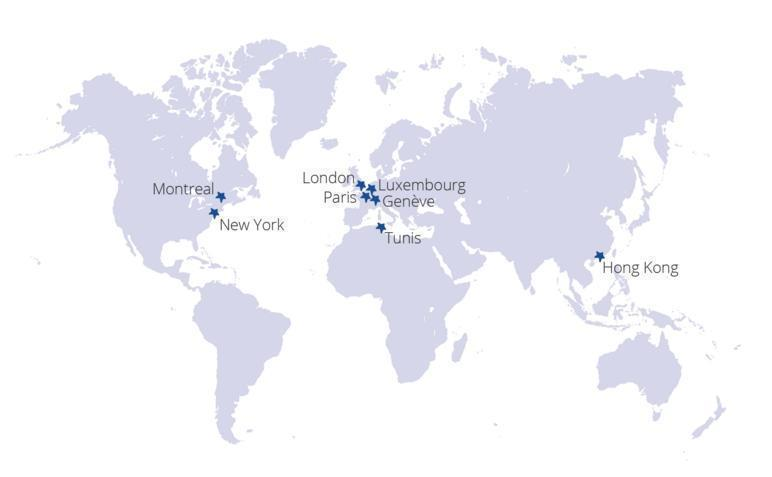
\includegraphics[scale=0.6]{img/talan1.jpg}
\centering
\caption{Implantation de Talan dans le monde}
\label{fig:talan-monde}
\end{figure}
%%%%%%%%%%%%%%%%%%%%%%%%%%%%%%%%%%%%%%%%%%%%%%%%%%%%%%%%%%%%%%%%
\subsubsection{Secteurs d’activité}
Talan Tunisie couvre essentiellement :
\begin{itemize}
\item[•]  Le secteur de la finance à travers une collaboration avec des banques d’investissement et des sociétés d'assurances.
\item[•] Le secteur de la télécommunication à travers des projets destinés aux opérateurs télécom et un ensemble de fournisseurs d’accès à internet.
\item[•] Le secteur du transport et de la logistique.
\item[•] Le secteur de l’énergie à travers des projets de développement visant des opérateurs de services liés à l’électricité,au gaz,à l'eau, etc.
\end{itemize}
%%%%%%%%%%%%%%%%%%%%%%%%%%%%%%%%%%%%%%%%%%%%%%%%%%%%%%%%%%%%%%%%%
%\color{red}
\subsection{Contexte du projet}
%\color{red} Présenter un peut qu'est ce qu'un système ERP et son inmportance dans une entreprise puis mentionne que Talan utilise Byblos comme outil ERP \\\color{black}
Les entreprises utilisent un système \textbf{"Enterprise Ressource Planning"} (ERP) en tant que progiciel permettant la gestion de l’ensemble des processus opérationnels d’une entreprise en intégrant plusieurs modules de gestion : module RH, module de gestion des fournisseurs, module de gestion de la comptabilité$\dots$\\ 
Autrement dit, l’ERP représente la « colonne vertébrale » d’une entreprise. \textbf{Talan Tunisie} a fait le choix d’investir dans la refonte de son système ERP, appellé \textbf{BYBLOS}, dont nous allons présenter la version existante. Nous exposerons aussi ses limites et l'impact de son architecture monolithique pour justifier la migration vers une architecture microservices.
%%%%%%%%%%%%%%%%%%%%%%%%%%%%%%%%%%%%%%%%%%%%%%%%%%%%%%%%%%%
\subsubsection{Présentation de l'outil BYBLOS}
BYBLOS est un ERP développé par les équipes de Talan Tunisie consulting, contenant plusieurs modules à savoir:
%\color{red} \\Tu peux mettre ici une figure d'acceuil de l'outil.\\
%Explique le but de chaque module en une phrase comme celui de gestion de fournisseurs.
\color{black}
\begin{itemize}
    \item Un module de gestion des ressources humaines : qui gère les fiches RH du personnel, ainsi que les soldes de congés.
    \item Un module de gestion des candidats : qui gère les fiches des candidats et leurs entretiens.
    \item Un module de gestion des collaborateurs : qui gère les fiches des collaborateurs.
    \item Un module de gestion des fournisseurs: qui gère les données personnelles et la situation des fournisseurs.
    \item Un module de gestion des contrats : qui expose le type de contrats et leurs détails (date d'effet, date de fin, durée $\dots{}$).
    
\end{itemize}
Dans le cadre de ce projet, nous nous intéressons au module de \textbf{gestion des candidats}.
Cette solution existante, basée sur une architecture monolithique, est développée avec Java Entreprise Edition (JEE) et Java Server Faces (JSF).
%\color{red} \\Mentionnes que dans ton projet tu t'intéresses au module de gestion des candidats\color{black}
%\subsubsection{Problématique: Impact de l’architecture monolithique sur l’outil Byblos}
%en effet, la solution existante de Byblos présente plusieurs limites :
%\begin{itemize}
    %\item  Le fait que Byblos est constitué en un seul Bloc, à chaque modification, l'équipe opérationnelle doit redéployer toute l'application et donc il faut refaire les tests(test unitaire, test de régression et test fonctionnel) et la révision de la qualité du code de tout le projet.
    %\item le nombre énorme de classes et les milliers de lignes de code ajoutés à chaque modification, augmentent la complexité du projet et rend l'application nécessite plus de ressources matérielles ce qui est très coûteux.
    %\item A chaque fois où un nouveau développeur intègre l'équipe de développement, il lui faut plusieurs jours voir semaines pour comprendre le code.
%\end{itemize}
%\newpage
%%%%%%%%%%%%%%%%%%%%%%%%%%%%%%%%%%%%%%%%%%%%%%%%%%%%%%%%%%%
\section{Problématique}
%\color{red}Ajoutes une phrase introductive ici.
\color{black}Dans cette section, nous allons présenter l'architecture monolithique, ainsi que son impact sur l'outil BYBLOS. 
%En fin nous proposerons la solution.
%%%%%%%%%%%%%%%%%%%%%%%%%%%%%%%%%%%%%%%%%%%%%%%%%%%%%%%%%%%
%\subsection{Les architectures monolithiques}
%\color{red}Définis ici qu'est ce qu'une architecture monolithique (utilises des figures si c possible). Dans la sous-section suivante tu vas lister ses inconvénients majeurs et leur impact sur Byblos.
\color{black}
L'architecture monolithique est l'architecture traditionnelle où  toutes les tâches sont réalisées dans une seule et grande application. Tous les services individuels accèdent à une grande base de données et sont édités via une interface utilisateur, tous implémentés dans une seule application. 
\begin{figure}[H]
    \centering
    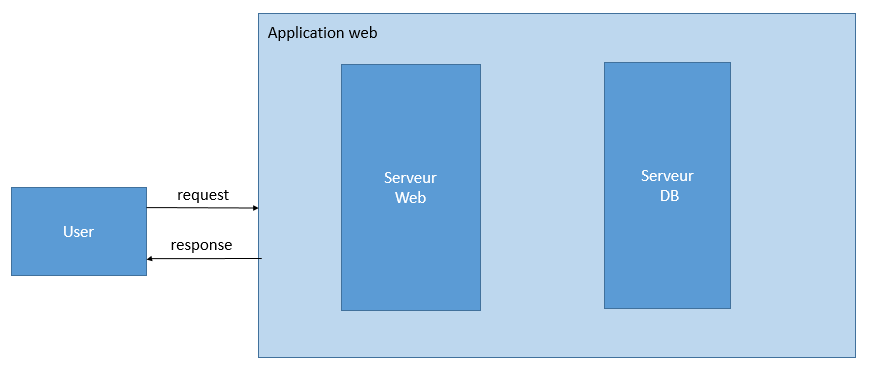
\includegraphics[scale=0.5]{img/archi mono.PNG}
    \caption{Architecture monolithique}
    \label{fig:Architecture monolitique}
\end{figure}

\color{black}
%\subsection{Impact de l’architecture monolithique sur l’outil Byblos}
Une architecture monolithique représente le modèle traditionnel unifié de conception d'un programme informatique. En se basant sur une telle architecture, la maintenance de l'outil BYBLOS est devenue trop difficile à cause de la complexité de l'application qui augmente à chaque itération.
%se base sur, rend la maintenance ou l'ajout d'un nouveau module très difficile due à la complexité du projet qui augmente à chaque itération.


%De plus, Le choix des technologies est décidé avant que le développement de l’application commence. Ainsi qu'une seule technologie est utilisée pour le développement de l’application.
En outre, une légère modification apportée à une petite partie de l’application nécessite la construction et le déploiement d'une version entièrement nouvelle et requiert une durée des tests automatiques et des builds plus longue, ce qui engendre un coût supplémentaire. De plus, l'application est constituée d'un seul bloc, un dysfonctionnement sur une partie du système affecte toute l’application. Cette architecture réduit l'agilité de l’équipe et la fréquence de livraison à cause du fort couplage entre les composants de l'application.\\
L'outil BYBLOS est une application web composée de trois couches comme le montre la Figure \ref{fig:architecure BYBLOS existante} :
\begin{itemize}
    \item \textbf{Couche présentation} : cette couche est composée des pages JSF et des servlets.
    \item \textbf{Couche métier} : cette couche représente l’ensemble métier de l’application. Elle est composée des EJBs.
    \item \textbf{Couche persistance} : c'est la couche Data Access Objects (DAO) qui transforme les objets métiers en données sérialisées, et inversement pour les échanges avec la base de donnée PostgreSql. Elle est réalisée en se basant sur le framework Hibernate/JPA.
\end{itemize}
\begin{figure}[H]
    \centering
    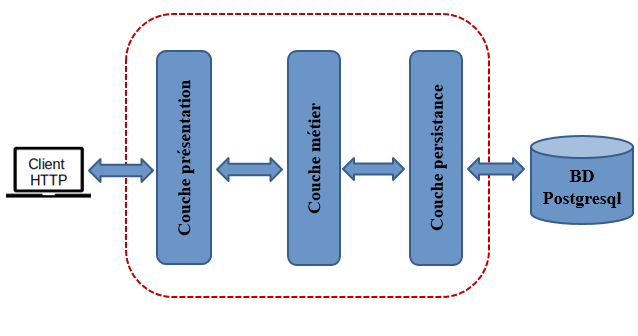
\includegraphics[scale=0.8]{img/archi mono byblos.PNG}
    \caption{Architecture monolithique de BYBLOS}
    \label{fig:architecure BYBLOS existante}
\end{figure}
% \begin{figure}[H]
%     \centering
%     \includegraphics[scale=0.5]{img/archit-mono.png}
%     \caption{Architecture monolithique de BYBLOS}
%     \label{fig:byblos_exist}
% \end{figure}
%%%%%%%%%%%%%%%%%%%%%%%%%%%%%%%%%%%%%%%%%%%%%%%%%%%%%%%%%%%%%%%%
\section{Solution proposée: Migration vers une architecture microservices}
\textbf{Talan} prévoit de renforcer son effectif d’ici fin 2020 en intégrant 3000 nouveaux collaborateurs et d’ouvrir, dès septembre 2020, un siège international à Londres ainsi que des bureaux à l’étranger, notamment en Belgique, en Italie et aux Pays-Bas.\\
De ce fait, le module de gestion des candidats dans l'ERP BYBLOS doit être disponible et performant à cette période. Après une étude approfondie de la solution existante, et dans le but de surmonter les limites de l'architecture monolithique ainsi que dans un souci de performance, l'équipe BYBLOS a décidé de faire une refonte de l'ERP BYBLOS existant vers une architecture microservices tout en améliorant les IHMs.\\
C'est dans ce cadre que s'inscrit notre projet de fin d'études, qui consiste à réaliser la migration du module de gestion des candidats de la solution existante vers une architecture microservices.\\
Notre travail consiste donc à :
\begin{itemize}
    \item Concevoir et implémenter le microservice de gestion des candidats;
    \item Enregistrer le microservice dans le  serveur de découverte (Eureka) et dans le Gateway (zuul);
    \item Ajouter le fichier de configuration du microservice dans le serveur de configuration.  
\end{itemize}
  
\color{black}
%%%%%%%%%%%%%%%%%%%%%%%%%%%%%%%%%%%%%%%%%%%%%%%%%%%%%%%%%%%%%%%
\section{Architecture microservices}

%\color{red}Ajoutes une phrase introductive ici
\color{black}
Dans cette section, nous définirons l'architecture microservices. Par la suite, nous allons présenter les caractéristiques d'un microservice, et enfin les avantages de cette architecture par rapport à l'architecture monolithique comme le montre la figure \ref{fig:architecture micro vs architecture mono}. \\
%\subsection{L'architecture microservices}
\begin{figure}[H]
    \centering
    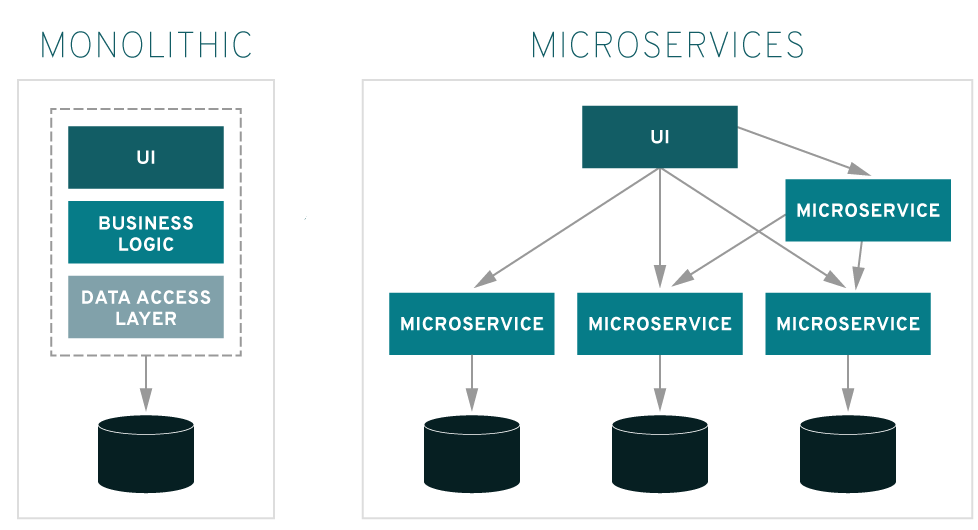
\includegraphics[scale=0.6]{img/monolithic-vs-microservices.png}
    \caption{Comparaison entre les architectures microservices et monolithique}
    \label{fig:architecture micro vs architecture mono}
\end{figure}

L'architecture microservices est une méthode distinctive de développement des systèmes logiciels, qui a connu une popularité grandissante ces dernières années. Il s'agit d'une méthode de développement d'applications logicielles en tant que suite de services modulables et indépendants.\\
Ce style d’architecture présente plusieurs avantages comme l’hétérogénéité technologique, la résistance contre l’échec, la scalabilité sur mesure, la facilité de déploiement, l’alignement organisationnel et la réutilisabilité.
%%%%%%%%%%%%%%%%%%%%%%%%%%%%%%%%%%%%%%%%%%%%%%%%%%%%%%%%%%%%%%%%
\subsection{Caractéristiques d'un microservice}
L’architecture microservices possède plusieurs caractéristiques qu’il est essentiel d’appliquer durant la conception et le développement d’une application basée sur les microservices.
\begin{enumerate}
    \item[1] \textbf{Concentration sur une seule fonctionnalité:}  Un microservice implémente une seule fonctionnalité dont il est responsable dans tout le système. Une fonctionnalité peut être une fonctionnalité métier contribuant à l’objectif du système, ou une fonctionnalité technique utilisée par plusieurs fonctionnalités métier.
    \item[2] \textbf{Déploiement individuel des microservices:} Chaque microservice doit être déployable indépendamment des autres. Ce point est important : tout changement ou mise à jour d'un microservice doivent être réalisés sans toucher aux autres microservices ni affecter leur exécution.\\
    Le système doit continuer à fonctionner correctement durant la mise à jour du microservice en question, ainsi qu'après l’avoir redéployé.
    \item[3] \textbf{Indépendance des microservices:} Un microservice peut correspondre à un ou plusieurs processus. Il doit être obligatoirement hébergé sur des processus indépendants. En d’autres termes, il ne doit pas partager un processus avec un autre microservice.\\
    En revanche, il peut être constitué de plusieurs processus, notamment dans le cas d'un accès à une base de données. Autrement dit, seul ce service peut accéder à cette base de données. C’est une façon d’éviter au maximum les interdépendances entre les microservices.\\
    Par exemple si on développe deux microservices sur le même processus, nous risquons d’avoir des interdépendances qui vont conduire à l’obligation de déployer les deux en même temps, ce qui est contradictoire avec les caractéristiques des microservices.
    \item[4] \textbf{Taille des microservices:} Comme l’indique le nom ”micro”, les microservices doivent être concentrés sur une seule et unique fonctionnalité, de façon à ce que leur développement et leur maintenance puisse se faire par des équipes de petites tailles.
    \item[5] \textbf{Remplaçabilité:} On doit pouvoir remplacer n’importe quel microservice du système dans un temps raisonnablement court.
    \item[6] \textbf{Conception pour l’échec:} L’un des atouts majeurs des microservices est qu’ils sont conçus pour être tolérants aux pannes. Dans une application en microservices, si un service échoue, les autres services ne sont pas affectés et adaptent leurs fonctionnements selon l’état du système dans lequel ils évoluent.
\end{enumerate}
%%%%%%%%%%%%%%%%%%%%%%%%%%%%%%%%%%%%%%%%%%%%%%%%%%%%%%%%%%%%%%%%
\subsection{Architecture monolithique Vs microservices}

Le tableau \ref{tab:comp} ci-dessous présente les principales différences entre les architectures microservice et monolithique.
\begin{longtable}[c]{
    |p{.20\textwidth}|
    |p{.35\textwidth}|
    |p{.35\textwidth}|
}
    \hline
    &    \textbf{Architecture Microservice}
    &    \textbf{Architecture Monolithique}\\
    \hline
    \textbf{Mise sur le marché}
    & Déploiement et mises à jour en microservices sont plus rapides et plus agiles.
    &Déploiement et mises à jour en un seul bloc, nécessitent plus de temps et sont moins agiles.    \\
    \hline
     \textbf{Haute évolutivité}
    & La possibilité d'étendre les déploiements sur plusieurs serveurs et infrastructures.
    &Le déploiement se fait sur un seul serveur.\\
    \hline
     \textbf{Résilience}
    & Les microservices sont indépandants. Lorsqu'un service tombe en panne, l'ensemble de l'application continue à fonctionner.
    & Lorsqu'un module tombe en panne, l'intégralité de l'application cesse de fonctionner.\\
    \hline
    \textbf{Facilité de déploiement}
    & Les applications basées sur des microservices sont plus modulaires et légères.
    &Les applications monolithiques sont déployées en un seul bloc et sont plus lourdes.\\
    \hline
    \textbf{Ouverture}
    & Les développeurs ont la liberté de choisir la technologie et le langage qui leur conviennent le mieux pour chaque fonction.
    &Les développeurs ne peuvent utiliser qu'une seule technologie et un seul langage pour toute l'application.\\
    \hline
\caption{Architecture microservices Vs monolithique}
\label{tab:comp}
\end{longtable} 
% \begin{itemize}
%     \item[-] \textbf{Mise sur le marché plus rapide}\\
% Comme les cycles de développement sont plus courts, l'architecture de microservices permet des déploiements et mises à jour plus agiles.
%     \item[-] \textbf{Haute évolutivité}\\
% À mesure que la demande pour certains services augmente, vous pouvez étendre les déploiements sur plusieurs serveurs et infrastructures pour répondre à vos besoins.
%     \item[-] \textbf{Résilience}\\
% Lorsqu'ils sont développés correctement, ces services indépendants n'ont aucun impact les uns sur les autres. Cela signifie que, lorsqu'un élément tombe en panne, l'ensemble de l'application ne cesse pas de fonctionner comme c'est le cas avec le modèle monolithique.
%     \item[-] \textbf{Facilité de déploiement}\\
% Les applications basées sur des microservices sont plus modulaires et légères que les applications monolithiques classiques. Aussi, vous pouvez les déployer plus sereinement. Certes, cela requiert une meilleure coordination, mais les bénéfices peuvent être énormes.
%     \item[-] \textbf{Accessibilité}\\
% Vu que l'application est décomposée en plusieurs éléments, les développeurs peuvent plus facilement comprendre, mettre à jour et améliorer chacun de ces éléments. Résultat : des cycles de développement plus courts, surtout s'ils sont associés à des méthodes de développement agiles.
%     \item[-] \textbf{Ouverture}\\
% Grâce aux API qui utilisent plusieurs langages, les développeurs ont la liberté de choisir la technologie et le langage qui conviennent le mieux à chaque fonction.
% \end{itemize}
%%%%%%%%%%%%%%%%%%%%%%%%%%%%%%%%%%%%%%%%%%%%%%%%%%%%%%%%%%%%%%%%
\section{Méthodologie de développement adoptée: Scrum}
Le choix de la méthodologie à utiliser durant le développement d'un logiciel doit répondre aux critères suivants :
\begin{itemize}
    \item[•] Exprimer au mieux les besoins des futurs clients.
    \item[•] Permettre de développer une application robuste et évolutive.
    \item[•] Élaborer une application qui répond aux besoins des clients dans des délais respectables.
\end{itemize}
Nous avons travaillé avec la méthode Scrum, déjà utilisée par l’équipe BYBLOS. Nous présentons, dans la suite, la méthode Scrum, les différents intervenants dans notre projet ainsi que son cycle de vie.
\subsection{Présentation de la méthode SCRUM}
Scrum est une méthode qui implémente les bonnes pratiques du Manifeste Agile dont l'utilisation s’étend au-delà du domaine informatique. Elle vise à produire les meilleurs logiciels possibles, le plus rapidement possible. Le cycle d'un projet Scrum est illustré dans la Figure  \ref{fig:scrum}.
\begin{figure}[H]
\centering
\frame{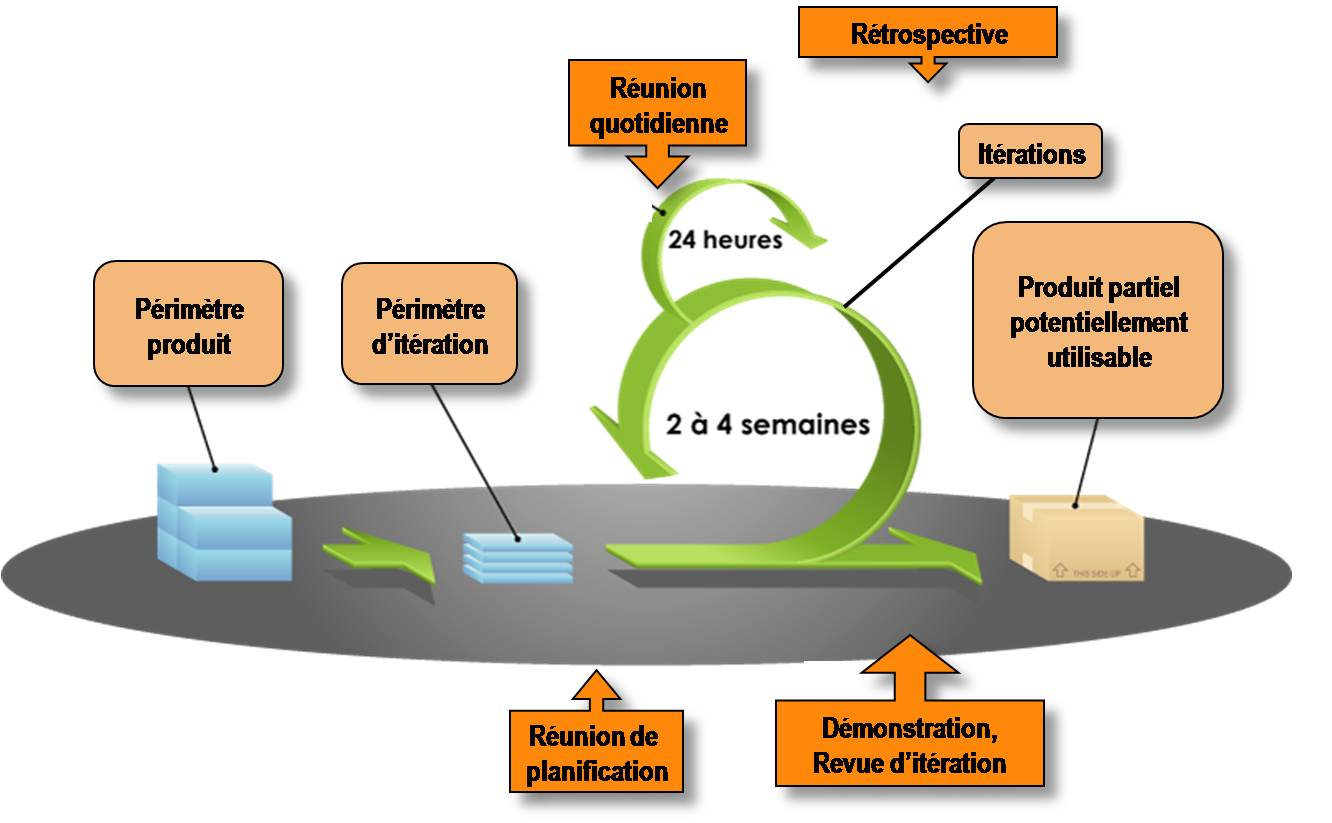
\includegraphics[scale=0.65]{img/cycle-scrum.jpg}}
\caption{Cycle de vie de SCRUM}
\label{fig:scrum}
\end{figure}
%%%%%%%%%%%%%%%%%%%%%%%%%%%%%%%%%%%%%%%%%%%%%%%%%%%%%%%%%%%%%%%
\subsection{Les rôles dans SCRUM}
La méthodologie SCRUM fait intervenir trois rôles principaux qui sont :
\begin{itemize}
    \item \textbf{Le Scrum Master:} C’est le coach de l’équipe, il assure plusieurs tâches : 
    \begin{itemize}
    \item Assister l’équipe pour appliquer la philosophie et les pratiques de Scrum.
    \item S’assurer que l’équipe bénéficie des meilleures conditions pour accomplir les tâches nécessaires.
    \item Surmonter les obstacles éventuels: prendre en compte les problèmes qui surviennent à tout moment sur le projet pour les éliminer.
    \item Faire en sorte que l’équipe reste concentrée sur le véritable objectif du projet, en s’assurant que chacun participe pleinement aux travaux de l’équipe.
\end{itemize}
    \item \textbf{Le Product Owner:} Il est le propriétaire du \textbf{Product Backlog}. Il représente les utilisateurs et est fortement impliqué dans les réunions de planification et d’avancement. Il a aussi la capacité d’annuler le sprint avant échéance.
    \item \textbf{La Scrum Team:} Il s’agit de l’équipe de développement. Elle produit chaque itération du projet, et ses membres sont les mêmes tout au long du projet.
\end{itemize}
%%%%%%%%%%%%%%%%%%%%%%%%%%%%%%%%%%%%%%%%%%%%%%%%%%%%%%%%%%%%%%%%
\subsection{Cycle de vie de Scrum}

\begin{itemize}
    \item [•]\textbf{ Backlog produit} : lister toutes les fonctionnalités en les triant par priorité.
    \begin{itemize}
    \item Besoins priorisés par le product owner. 
    \item Besoins évalués par l’équipe.
\end{itemize}
    \item [•] \textbf{Backlog de sprint} : extraire les fonctionnalités qui vont être développées au prochain sprint.
    \begin{itemize}
    \item Extrait du backlog produit.
    \item Besoins éclatés en tâches.
\end{itemize}
    \item [•] \textbf{Sprint} : la scrum team commence à developper les fonctionnalités du Sprint
    \begin{itemize}
    \item Développement des fonctionnalités du backlog de sprint. 
    \item Aucune modification du backlog de sprint possible.
\end{itemize}
    \item [•] \textbf{Mêlée quotidienne} : une petite réunion journalière pour identifier les problèmes rencontrés par chaque membre de l'équipe de développement.
    \begin{itemize}
    \item Point de contrôle quotidien de l’équipe. 
    \item Interventions régulées : 2 minutes par personne.
\end{itemize}
    \item [•] \textbf{Incrément logiciel} : Après avoir achevé le sprint et testé les fonctionnalités, un livrable est prêt à être déployé. 
    \begin{itemize}
    \item Livrable remis au Product Owner à la fin du sprint. 
\end{itemize}
\end{itemize}


\section*{Conclusion}
Dans ce chapitre, nous avons défini le cadre général de notre projet, en présentant l'organisme d'accueil et la solution proposée. Nous avons aussi défini les principales notions qui constituent la base de ce travail. Le prochain chapitre sera consacré à la spécification des besoins fonctionnels et non-fonctionnels de notre système.
        \clearpage
        
        \chapter{Analyse et spécification des besoins}

\section*{Introduction}
Dans toute application informatique, les fonctionnalités doivent être mises en relation avec un ensemble de besoins définis par l'utilisateur du système. Les fonctions que le système est appelé à accomplir découlent essentiellement des besoins exprimés. La spécification des besoins constitue l'élément de base sur lequel sera construite l’architecture du système. Nous commencerons par identifier les acteurs du système. Nous définirons ensuite les besoins exprimés par ces derniers, et à partir desquels serons définis les cas d’utilisations de l'application.
%Dans ce chapitre nous nous intéressons par la phase spécification et analyse des besoins qui représente la base de départ de notre travail. Notre objectif ici est de dégager les différents acteurs ainsi que de spécifier et analyser les besoins fonctionnels et non fonctionnels relatifs au système. Nous finissons par présenter quelques diagrammes de cas d’utilisation afin d’expliquer approfondissement les besoins.
%%%%%%%%%%%%%%%%%%%%%%%%%%%%%%%%%%%%%%%%%%%%%%%%%%%%%%%%%%%
\section{Identification des acteurs}
Un acteur est l'idéalisation d'un rôle joué par une entité distincte du système et qui interagit directement avec lui. Notre module comporte deux acteurs majeurs:
 \begin{itemize} 
    \item  \textbf{ Le Back-office} : cet acteur est responsable de la gestion de la fiche du candidat et de l'assignation d'un entretien à un recruteur.
    \item  \textbf{Le recruteur} : c'est celui qui va passer l'entretien d'embauche au candidat.
 \end{itemize}
%%%%%%%%%%%%%%%%%%%%%%%%%%%%%%%%%%%%%%%%%%%%%%%%%%%%%%%%%%%
\section{Identification des besoins}
L’application offre à chaque acteur un ensemble de fonctionnalités. Cette partie sera donc consacrée aux besoins fonctionnels et non fonctionnels relatifs à l’application.
%%%%%%%%%%%%%%%%%%%%%%%%%%%%%%%%%%%%%%%%%%%%%%%%%%%%%%%%%%%
\subsection{Les besoins fonctionnels}
Dans cette partie, nous citons les fonctionnalités pour chaque acteur.
\begin{itemize}
    \item [•]Pour le back-office, l'application doit lui permettre de:   
 \begin{itemize}
     \item Gérer une fiche candidat : le back-office peut ajouter ou modifier une fiche candidat.
     \item Gérer un entretien : le back-office peut planifier un entretien, modifier certains de ses éléments ou consulter son Workflow(historique).
     \item Rechercher un candidat : le back-office peut rechercher un candidat selon plusieurs critères. 
     \item Consulter le KPI des avis des entretiens : le back-office peut consulter le graphe(en secteurs) qui indique le nombre total,par année, de candidats correspondant à chacun des avis listés.
 \end{itemize}
    \item [•] Pour le recruteur , l'application doit lui permettre de : 
 \begin{itemize}
     \item Modifier un entretien : le recruteur peut modifier certains éléments de l'entretien.
     \item Rechercher un candidat : le recruteur peut rechercher un candidat selon plusieurs critères.
     \item Valider un entretien : le recruteur peut accepter ou rejeter un entretien selon sa disponibilité.
     \item Consulter le KPI des avis des entretiens : le recruteur peut consulter le graphe(en secteurs) qui indique le nombre total,par année, de candidats correspondant à chacun des avis listés.
 \end{itemize}
\end{itemize}


%%%%%%%%%%%%%%%%%%%%%%%%%%%%%%%%%%%%%%%%%%%%%%%%%%%%%%%%
 \subsection{Les besoins non fonctionnels}
Dans l’intention de réussir notre tâche, l’application doit vérifier quelques propriétés et doit tenir compte de certaines contraintes et exigences:
 \begin{itemize}
     \item  \textbf{Ergonomie:} les interfaces graphiques de notre module de gestion des candidats doit avoir une ergonomie identique à celle des modules déjà migrés vers l'architecture microservices.
     \item \textbf{Sécurité:} notre application doit assurer la sécurité pour chaque authentification.
    \item \textbf{Maintenabilité:} notre module de gestion des candidats doit être évolutif et extensible.
 \end{itemize}
%%%%%%%%%%%%%%%%%%%%%%%%%%%%%%%%%%%%%%%%%%%%%%%%%%%%%%%%%
 \section{Diagramme de cas d'utilisation global}
Cette partie permet de montrer le comportement de l'application. Nous utilisons le diagramme de cas d'utilisation pour visualiser les fonctionnalités du système et les interactions entre les acteurs et le système.

La Figure \ref{fig:cas_utilisation_global} présente le diagramme des cas d'utilisation global de notre application montrant les fonctionnalités offertes pour chacun des deux principaux acteurs(back-office et recruteur).
 
 \begin{figure}[H]
     \centering
     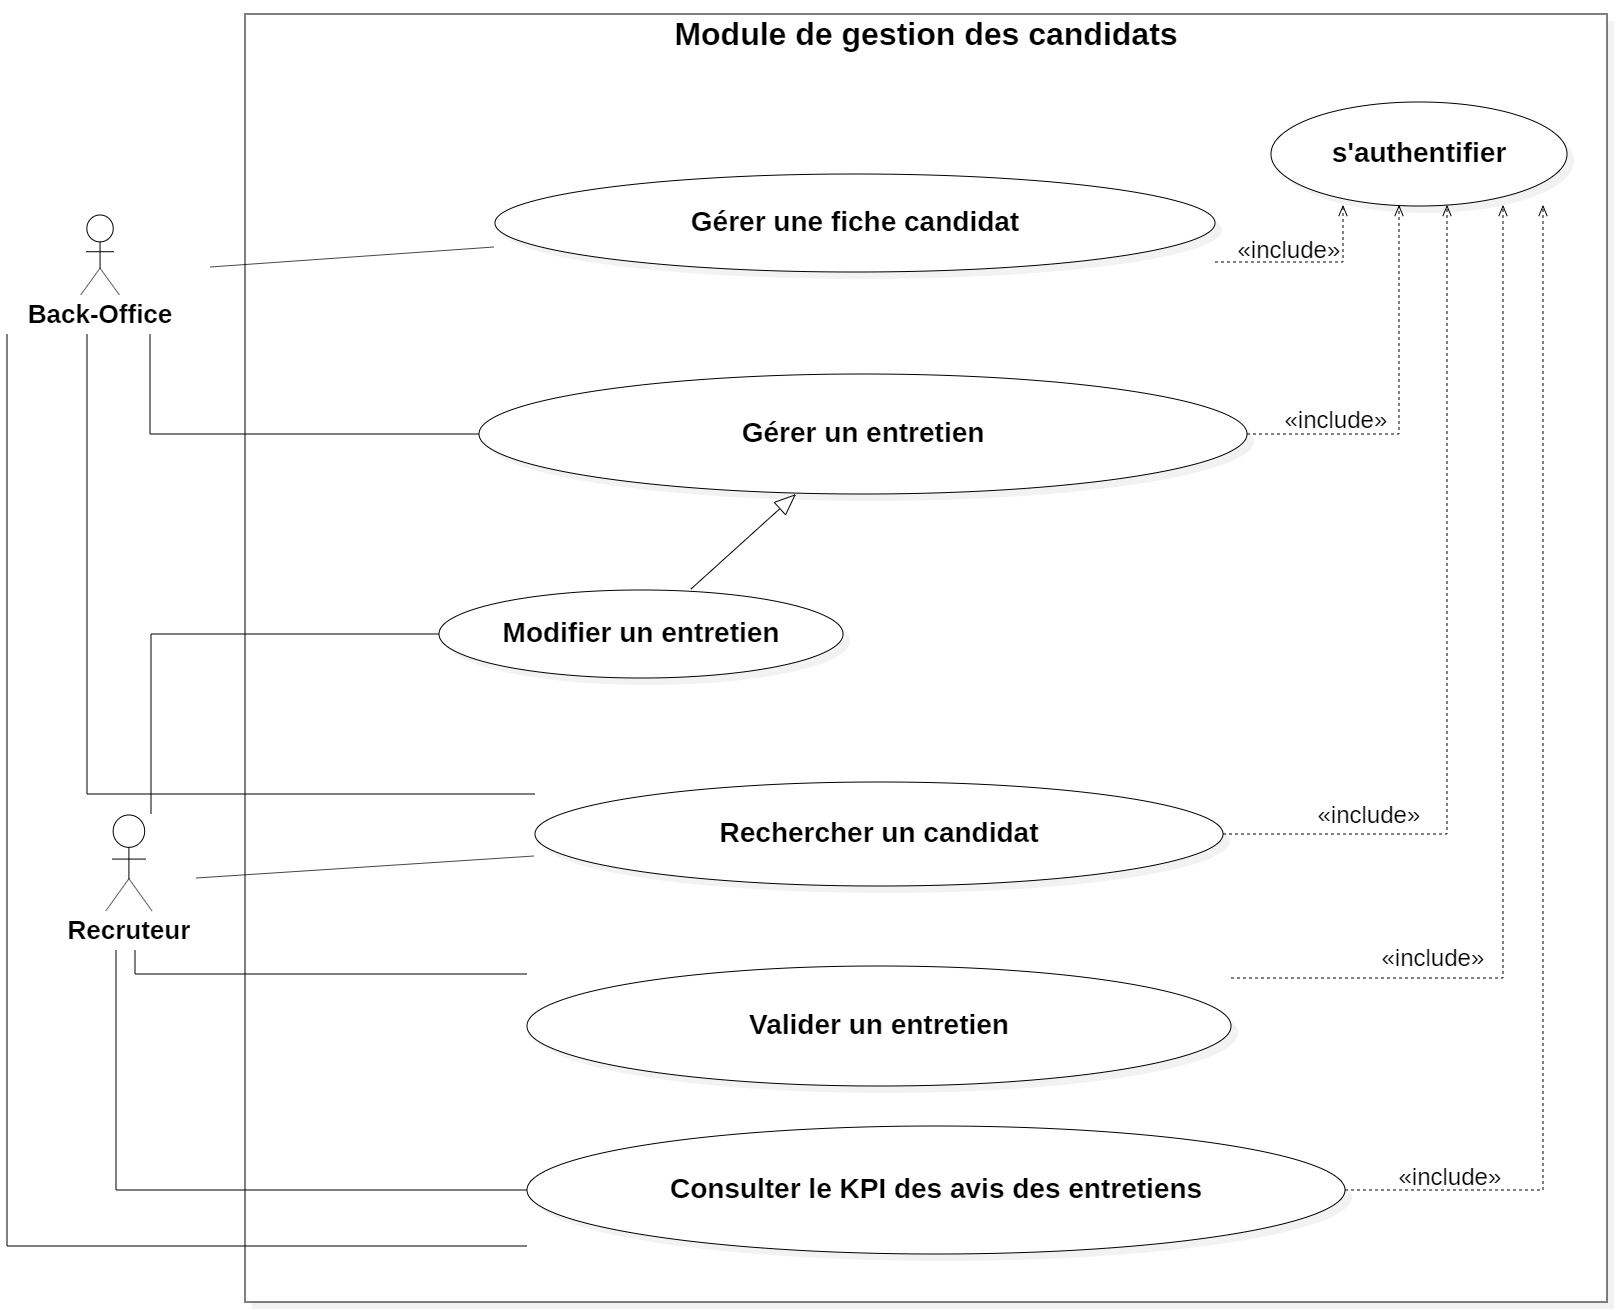
\includegraphics[scale=0.4]{img/UseCaseDiagramv4.png}
     \caption{Diagramme de cas d'utilisation global}
     \label{fig:cas_utilisation_global}
 \end{figure}
Nous présentons dans la suite le raffinement des cas d'utilisation pour chaque acteur.
%%%%%%%%%%%%%%%%%%%%%%%%%%%%%%%%%%%%%%%%%%%%%%%%%%%%%%%%
\section{Diagrammes des cas d'utilisation détaillés}
Dans cette section nous présentons, pour chaque acteur, les diagrammes des cas d'utilisation détaillés et leur description textuelle.
%%%%%%%%%%%%%%%%%%%%%%%%%%%%%%%%%%%%%%%%%%%%%%%
\subsection{Raffinement des cas d'utilisation pour le back-office}
Dans cette partie, nous développons chaque cas d'utilisation du back-office avec une description détaillée.
%%%%%%%%%%%%%%%%%%%%%%%%%%%%%%%%%%%%%%%%
\subsubsection{Cas d'utilisation "Gérer une fiche candidat"}
Nous nous intéressons, dans cette partie, au raffinement du cas d'utilisation "Gérer une fiche candidat". Les fonctionnalités relatives à ce diagramme sont présentées dans la Figure \ref{fig:raffinement_fiche_candidat}.
\begin{figure}[H]
     \centering
     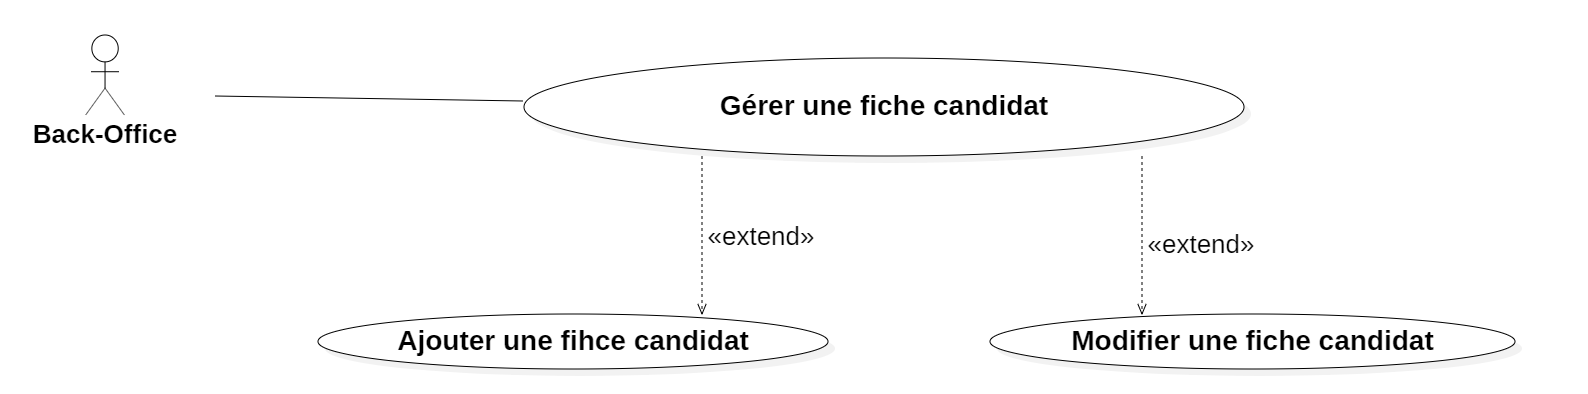
\includegraphics[scale=0.35]{img/raffinement fiche candidat.png}
     \caption{Diagramme de cas d'utilisation "Gérer une fiche candidat"}
     \label{fig:raffinement_fiche_candidat}
 \end{figure}
Nous détaillons dans ce qui suit les deux cas d'utilisation : "Ajouter une fiche candidat" et "Modifier une fiche candidat". Après authentification, le back-office peut toujours créer une nouvelle fiche candidat.
\begin{longtable}[c]{
    |p{.20\textwidth}|
    |p{.70\textwidth}|
}
    \hline
    \textbf{Titre}
    &    Ajouter une fiche candidat\\
    \hline
    \textbf{Résumé}
    & Le back-office peut ajouter une nouvelle fiche candidat. \\
    \hline
     \textbf{Pré-condition}
    & Le back-office doit être authentifié.\\
    \hline
     \textbf{Scénario normal}
    & \begin{itemize}
        \item A1 : Le back office clique sur le bouton "Ajouter fiche candidat".
        \item A2 : Le système affiche le formulaire à remplir.
        \item A3 : Le back-office introduit les informations nécessaires.
        \item A4 : Le système vérifie les informations saisies et ajoute le candidat.
    \end{itemize}\\
    \hline
    \textbf{Enchaînement d'erreur}
    & E1 : Le système affiche un message d'erreur mentionnant la présence d'un champ obligatoire vide.\\
    \hline
    \textbf{Post-condition}
    & Une nouvelle fiche candidat est ajoutée.\\
    \hline
\caption{Description du cas d'utilisation "Ajouter une fiche candidat"}
\label{tab:desc_ajout_fiche}
\end{longtable} 
\newpage
Le back-office peut aussi modifier une fiche candidat.
\begin{longtable}[c]{
    |p{.20\textwidth}|
    |p{.70\textwidth}|
}
    \hline
    \textbf{Titre}
    &    Modifier une fiche candidat\\
    \hline
    \textbf{Résumé}
    & Le back-office peut modifier une fiche candidat déjà créée. \\
    \hline
     \textbf{Pré-condition}
    & Le back-office doit être authentifié.\\
    \hline
     \textbf{Scénario normal}
    & \begin{itemize}
        \item A1 : Une fois la recherche est effectuée, le back office clique sur le bouton "Consulter ou Modifier une fiche candidat" pour le candidat choisis. 
        \item A2 : Le système affiche le formulaire contenant les informations du candidat concerné.
        \item A3 : Le back-office modifie les informations nécessaires.
        \item A4 : Le système vérifie les informations saisies et enregistre les modifications.
    \end{itemize}\\
    \hline
    \textbf{Enchaînement d'erreur}
    & E1 : Le système affiche un message d'erreur mentionnant la présence d'un champ obligatoire vide.\\
    \hline
    \textbf{Post-condition}
    & Une fiche candidat est modifiée.\\
    \hline
\caption{Description du cas d'utilisation "Modifier une fiche candidat"}
\label{tab:desc_modif_fiche}
\end{longtable} 
%%%%%%%%%%%%%%%%%%%%%%%%%%%%%%%%%%%%%%%%%%%%%%%%
\subsubsection{Cas d'utilisation "Gérer un entretien"}
Dans cette partie, nous nous concentrons sur le raffinement du cas d'utilisation "Gérer un entretien". Les fonctionnalités relatives à ce diagramme sont représentées dans la Figure \ref{fig:gerer_entretien}.

\begin{figure}[H]
     \centering
     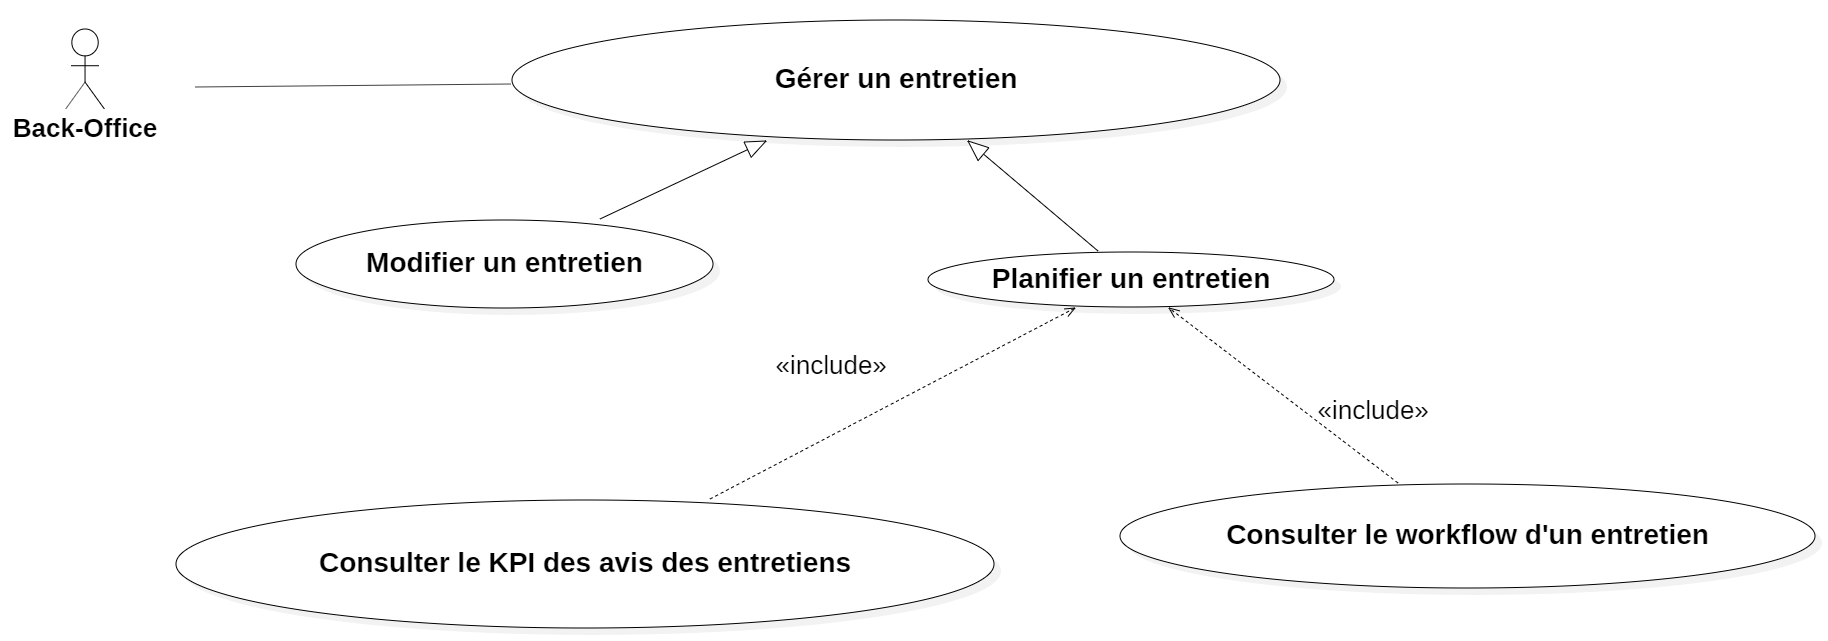
\includegraphics[scale=0.35]{img/raffinement gerer entretien.png}
     \caption{Diagramme de cas d'utilisation "Gérer un entretien"}
     \label{fig:gerer_entretien}
 \end{figure}

Nous détaillons dans ce qui suit les quatres cas d'utilisation : "Planifier un entretien" , "Modifier un entretien", "Consulter le KPI des avis des entretiens" et "Consulter le workflow d'un entretien". Le back-office peut toujours planifier un entretien après avoir été authentifié.
\begin{longtable}[c]{
    |p{.20\textwidth}|
    |p{.70\textwidth}|
}
    \hline
    \textbf{Titre}
    &   Planifier un entretien\\
    \hline
    \textbf{Résumé}
    & Le back-office peut planifier un nouvel entretien. \\
    \hline
     \textbf{Pré-condition}
    & Le back-office doit être authentifié.\\
    \hline
     \textbf{Scénario normal}
    & \begin{itemize}
        \item A1 : Une fois la fiche du candidat est créée, le back-office clique sur le bouton "Planifier un entretien". 
        \item A2 : Le système affiche le formulaire de l'entretien.
        \item A3 : Le back-office introduit les informations nécessaires de l'entretien.
        \item A4 : Le back-office clique sur le bouton "Enregistrer".
        \item A5 : Le système vérifie les informations saisies et ajoute l'entretien.
        \item A6 : Le système attribue le statut "En attente" pour cet entretien.
        \item A7 : Le système envoie un e-mail, généré automatiquement, au recruteur sélectionné, contenant la date, l'heure, les nom et prénom du candidat et un lien qui mène vers la fiche de ce candidat.
    \end{itemize}\\
    \hline
    \textbf{Enchaînement d'erreur}
    & E1 : Le système affiche un message d'erreur mentionnant la présence d'un champ obligatoire vide.\\
    \hline
    \textbf{Post-condition}
    & Un nouvel entretien est ajouté.\\
    \hline
\caption{Description du cas d'utilisation "Planifier un entretien"}
\label{tab:desc_planif_entretien}
\end{longtable} 
Le back-office peut aussi modifier un entretien.
\begin{longtable}[c]{
    |p{.20\textwidth}|
    |p{.70\textwidth}|
}
    \hline
    \textbf{Titre}
    &   Modifier un entretien\\
    \hline
    \textbf{Résumé}
    & Le back-office peut modifier un entretien déjà planifié. \\
    \hline
     \textbf{Pré-condition}
    & Le back-office doit être authentifié.\\
    \hline
     \textbf{Scénario normal}
    & \begin{itemize}
        \item A1 : Une fois un entretien est créé, le back-office clique sur le bouton "Modifier un entretien". 
        \item A2 : Le système affiche le formulaire de l'entretien déjà créé.
        \item A3 : Le back-office introduit les modifications d'informations nécessaires.
        \item A4 : Le back-office clique sur le bouton "Enregistrer".
        \item A5 : Le système vérifie les informations saisies et enregistre les modifications.
    \end{itemize}\\
    \hline
    \textbf{Enchaînement d'erreur}
    & E1 : Le système affiche un message d'erreur mentionnant la présence d'un champ obligatoire vide.\\
    \hline
    \textbf{Post-condition}
    & Un entretien est modifié.\\
    \hline
\caption{Description du cas d'utilisation "Modifier un entretien"}
\label{tab:desc_modif_entretien}
\end{longtable} 

Le back-office peut aussi consulter le KPI des avis des recruteurs lors des entretiens,sachant que ces avis changent d'une implantation à une autre de Talan après qu'un entretien ait été planifié.
\begin{longtable}[c]{
    |p{.20\textwidth}|
    |p{.70\textwidth}|
}
    \hline
    \textbf{Titre}
    &   Consulter le KPI des avis des recruteurs lors des entretiens\\
    \hline
    \textbf{Résumé}
    & Le back-office peut consulter le KPI des avis des entretiens. \\
    \hline
     \textbf{Pré-condition}
    & Le back-office doit être authentifié et l'entretien déjà créé.\\
    \hline
     \textbf{Scénario normal}
    & \begin{itemize}
        \item A1 : Le back-office navigue vers l'interface d'accueil(Dashboard). 
        \item A2 : Le système affiche l'interface contenant un graphe à secteurs montrant le nombre total de candidats par avis(qui concerne l'implantation de Talan du back-office connecté) pour une année sélectionnée au préalable.
    \end{itemize}\\
    \hline
    \textbf{Enchaînement d'erreur}
    & \\
    \hline
    \textbf{Post-condition}
    & Le KPI des avis des entretiens est consulté.\\
    \hline
\caption{Description du cas d'utilisation "Consulter le KPI des avis des entretiens"}
\label{tab:desc_consult_KPI}
\end{longtable} 

Le back-office peut aussi consulter le Workflow d'un entretien qui représente son historique:
\begin{itemize}
    \item \textbf{Au niveau du back-office} : la date de création de l'entretien, les nom et prénom de l'intervenant au back-office qui a créé l'entretien.
    \item \textbf{Au niveau du recruteur} : après l'acceptation ou le rejet de l'entretien par ce dernier : la date de la décision du recruteur, les nom et prénom de celui-ci.
\end{itemize} 
\begin{longtable}[c]{
    |p{.20\textwidth}|
    |p{.70\textwidth}|
}
    \hline
    \textbf{Titre}
    &   Consulter le Workflow d'un entretien\\
    \hline
    \textbf{Résumé}
    & Le back-office peut consulter le workflow d'un entretien déjà créé. \\
    \hline
     \textbf{Pré-condition}
    & Le back-office doit être authentifié et un entretien déjà créé.\\
    \hline
     \textbf{Scénario normal}
    & \begin{itemize}
        \item A1 : Une fois un entretien est créé, le back-office clique sur le bouton "Consulter Workflow" 
        \item A2 : Le système affiche un modal ( Popup: une petite fenêtre) contenant la date de création , les nom et prénom de l'intervenant au back-office qui a créé l'entretien, ainsi que la date de l'acceptation ou du rejet de l'entretien avec le nom et le prénom du recruteur concerné.
    \end{itemize}\\
    \hline
    \textbf{Enchaînement d'erreur}
    & \\
    \hline
    \textbf{Post-condition}
    & La fenêtre du Workflow est affichée.\\
    \hline
\caption{Description du cas d'utilisation "Consulter le workflow d'un entretien"}
\label{tab:desc_consult_workflow}
\end{longtable} 
\subsection{Raffinement des cas d'utilisation pour le recruteur}
Nous développons, dans cette partie, chaque cas d'utilisation du recruteur avec une description détaillée.
\subsubsection{Cas d'utilisation "Valider un entretien"}
Nous nous intéressons, dans cette partie, au raffinement du cas d'utilisation "Valider un entretien". Les fonctionnalités relatives à ce diagramme sont représentées dans la Figure \ref{fig:valid_entretien}
\begin{figure}[H]
     \centering
     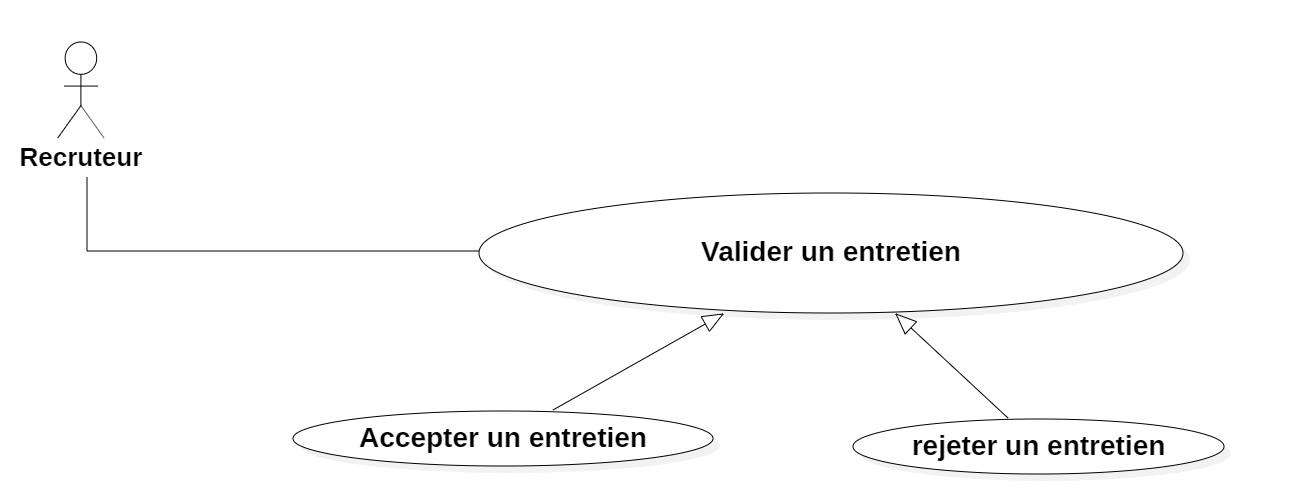
\includegraphics[scale=0.35]{img/raffinement valider un entretien.png}
     \caption{Diagramme de cas d'utilisation "Valider un entretien"}
     \label{fig:valid_entretien}
 \end{figure}
 Nous détaillons dans ce qui suit les deux cas d'utilisation : "Accepter un entretien" et "Rejeter un entretien". Après la planification d'un entretien et l'authentification du recruteur, un e-mail généré automatiquement sera envoyé à ce dernier pour lui notifier qu'un entretien est prévu à une date et à une heure précises, et lui transmettre un lien vers la fiche du candidat sur laquelle il indique sa décision d'accepter ou de rejeter l'entretien.
 \begin{longtable}[c]{
    |p{.20\textwidth}|
    |p{.70\textwidth}|
}
    \hline
    \textbf{Titre}
    &   Accepter un entretien\\
    \hline
    \textbf{Résumé}
    & Le recruteur peut accepter un entretien déjà créé. \\
    \hline
     \textbf{Pré-condition}
    & Le recruteur doit être authentifié et un entretien déjà créé.\\
    \hline
     \textbf{Scénario normal}
    & \begin{itemize}
        \item A1 : Une fois un entretien est créé et l'e-mail est envoyé, le recruteur clique sur le lien dans l'e-mail et l'interface de la fiche du candidat sera chargée. 
        \item A2 : le recruteur clique sur le bouton "Accepter un entretien".
        \item A3 : Le système modifie le statut de l'entretien de "En attente" en "Accepté".
    \end{itemize}\\
    % \hline
    % \textbf{Enchaînement d'erreur}
    % & \\
    \hline
    \textbf{Post-condition}
    & Le statut de l'entretien est modifié en "Accepté"\\
    \hline
\caption{Description du cas d'utilisation "Accepter un entretien"}
\label{tab:accept_entretien}
\end{longtable}
 Le recruteur peut aussi rejeter un entretien.
 \newpage
  \begin{longtable}[c]{
    |p{.20\textwidth}|
    |p{.70\textwidth}|
}
    \hline
    \textbf{Titre}
    &   Rejeter un entretien\\
    \hline
    \textbf{Résumé}
    & Le recruteur peut rejeter un entretien déjà créé. \\
    \hline
     \textbf{Pré-condition}
    & Le recruteur doit être authentifié et un entretien déjà créé.\\
    \hline
     \textbf{Scénario normal}
    & \begin{itemize}
        \item A1 : Une fois un entretien est créé et l'e-mail est envoyé, le recruteur clique sur le lien dans l'e-mail et l'interface de la fiche du candidat sera chargée. 
        \item A2 : le recruteur clique sur le bouton "Rejeter un entretien".
        \item A3 : Le système modifie le statut de l'entretien de "En attente" en "Rejeté".
    \end{itemize}\\
    %\hline
    % \textbf{Enchaînement d'erreur}
    % & \\
    \hline
    \textbf{Post-condition}
    & Un e-mail est envoyé au back-office pour le notifier.\\
    \hline
\caption{Description du cas d'utilisation "Rejeter un entretien"}
\label{tab:rejet_entretien}
\end{longtable}
%%%%%%%%%%%%%%%%%%%%%%%%%%%%%%%%%%%%%%%%%%%%%%%
\subsubsection{Cas d'utilisation "Rechercher un candidat"}
Dans cette partie, nous nous intéressons au raffinement du cas d'utilisation "Rechercher un candidat". Les fonctionnalités relatives à ce diagramme sont représentées dans la figure \ref{fig:recherche_candidat}.
\begin{figure}[H]
     \centering
     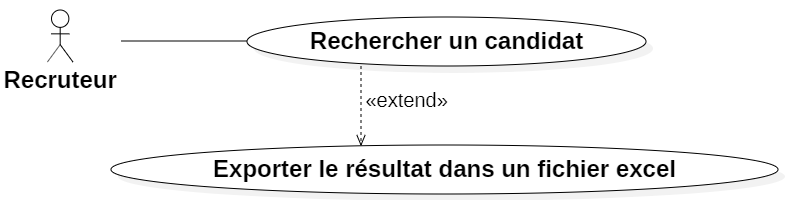
\includegraphics[scale=0.6]{img/raffinement recherche candidat.png}
     \caption{Diagramme de cas d'utilisation "Rechercher un candidat"}
     \label{fig:recherche_candidat}
 \end{figure}
 Nous détaillons dans ce qui suit le cas d'utilisation "Exporter le résultat dans un fichier excel". Après que le recruteur ait effectué une recherche des candidats, le résultat est affiché sous forme d'un tableau. Le recruteur peut sélectionner un ou plusieurs candidats dans le tableau, et clique sur le bouton "Exporter" pour télécharger un fichier excel qui contient toutes les informations concernant les candidats sélectionnés. 
 \newpage
   \begin{longtable}[c]{
    |p{.20\textwidth}|
    |p{.70\textwidth}|
}
    \hline
    \textbf{Titre}
    &   Exporter le résultat dans un fichier excel\\
    \hline
    \textbf{Résumé}
    & Le recruteur peut exporter le résultat de la recherche de candidats dans un fichier excel. \\
    \hline
     \textbf{Pré-condition}
    & Le recruteur doit être authentifié et une recherche doit être effectuée.\\
    \hline
     \textbf{Scénario normal}
    & \begin{itemize}
        \item A1 : Une fois la recherche est effectuée, le recruteur sélectionne le(s) candidat(s) en cliquant sur la case à cocher pour chaque candidat. 
        \item A2 : le recruteur clique sur le bouton "Exporter".
        \item A3 : Le système génère un fichier excel contenant toutes les informations relatives aux candidats sélectionnés, et le télécharge à travers le navigateur .
    \end{itemize}\\
    % \hline
    % \textbf{Enchaînement d'erreur}
    % & \\
    %
    \hline
    \textbf{Post-condition}
    & Un fichier excel est téléchargé.\\
    \hline
\caption{Description du cas d'utilisation "Exporter le résultat dans un fichier excel"}
\label{tab:recherche_candidat}
\end{longtable}
\section*{Conclusion}
Dans ce chapitre, nous avons mis en évidence les acteurs, ainsi que les besoins fonctionnels et non fonctionnels du système.
D'autre part, nous avons détaillé les différents cas d'utilisation en précisant une description textuelle pour chaque cas. En effet, ce chapitre nous a permis de mieux comprendre les fonctionnalités à développer. L'étape suivante concerne la conception de notre application qui sera présenté dans le prochain chapitre.


        \clearpage
        
        \chapter{Conception}
%%%%%%%%%%%%%%%%%%%%%%%%%%%%%%%%%%%%%%%%%%%%%%%%%%%%%%
\section*{Introduction}
Ce chapitre est consacré, en premier lieu, à visualiser la conception générale de l'application en particulier son architecture logique. En deuxième lieu, nous présenterons l’enchaînement de conception qui a pour but de mieux expliciter les fonctionnalités en se basant sur les diagrammes de séquences. L’objectif recherché étant de façonner le système et de lui donner une forme répondant à tous les besoins et exigences recensés.
%%%%%%%%%%%%%%%%%%%%%%%%%%%%%%%%%%%%%%%%%%%%%%%%%%%%%%%
\section{Conception générale}
Dans cette section, nous présentons, en premier lieu, les interactions des composants de notre application dans un diagramme de déploiement. En deuxième lieu, nous exposons l'architecture logique ainsi que le diagramme de paquetage. 
%%%%%%%%%%%%%%%%%%%%%%%%%%%%%%%%%%%%%%%%%%%%%%%%%%%%%%
\subsection{Diagramme de déploiement de l'application}
La Figure \ref{fig:diagram_deploiement} décrit l'infrastructure selon laquelle notre application est déployée. Cette infrastructure est constituée des éléments suivants :
\begin{itemize}
    \item \textbf{Serveur web} : il contient un seul composant "Angular Frontend" qui est la partie forntend de notre application.
    \item \textbf{Serveur} : il contient plusieurs composants : 
    \begin{itemize}
        \item \textbf{Gateway}: c'est le composant qui est responsable de l'acheminement des requêtes reçues du serveur web vers les différents microservices, dont le module "Gestion Candidat".
        \item \textbf{Eureka discovery service}: c'est un service de découverte des microservices qui permet de signaler un microservice défectueux.
        \item \textbf{Configuration} : c'est le composant qui contient toute la configuration des différents microservices.
        \item \textbf{Gestion candidat} : c'est le microservice objet de ce travail qui est composé principalement de trois parties : 
        \begin{itemize}
            \item G\textbf{estion candidat Controller} : qui contient les différents web services REST.
            \item \textbf{Gestion candidat Service} : qui contient le métier de notre module.
            \item \textbf{Gestion candidat DAO} : qui contient la partie de persistance des données dans la base de données.
        \end{itemize}
    \end{itemize}
    \item \textbf{Serveur Base de données} : il contient un seul composant, qui est le Système de gestion de base de données Postgresql.
\end{itemize}
\begin{figure}[H]
     \centering
     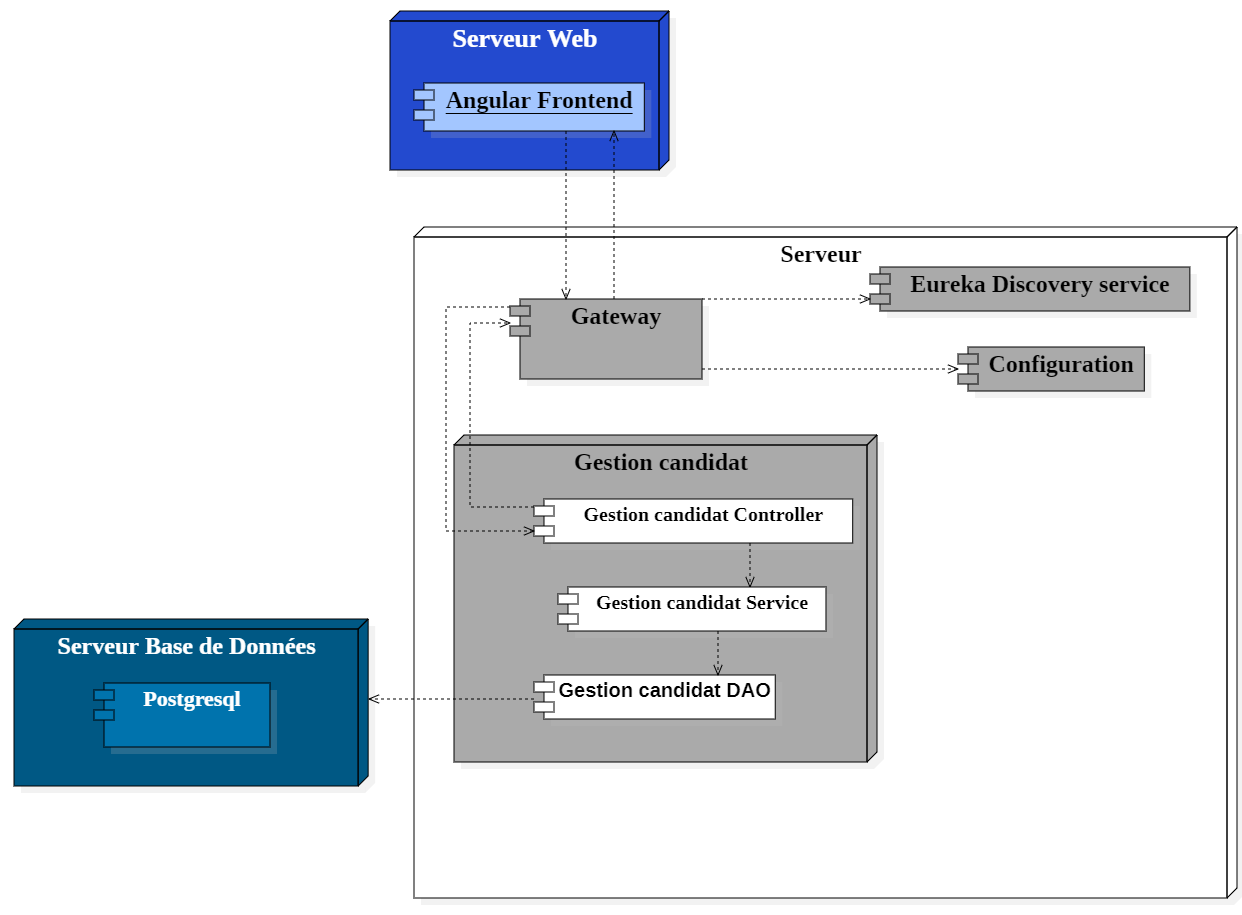
\includegraphics[scale=0.5]{img/DeploymentDiagram1.png}
     \caption{Diagramme de déploiement de l'application}
     \label{fig:diagram_deploiement}
 \end{figure}
%%%%%%%%%%%%%%%%%%%%%%%%%%%%%%%%%%%%%%%%%%%%%%%%%%%%%%
 \subsection{Architecture logique de l'application}
 L’architecture logique décrit les différentes couches d’une application, leurs interrelations et leurs interactions. Notre module de gestion des candidats est composé des couches suivantes présentées dans la Figure \ref{fig:archi_logique}.
 \begin{itemize}
     \item \textbf{Couche présentation} : cette couche contient les interfaces graphiques qui permettent la visualisation des données pour l'utilisateur.
     \item \textbf{Couche contrôleur} : cette couche contient les différents web services REST qui permettent de relier la couche présentation avec la partie métier de notre application.
     \item \textbf{Couche Service} : cette couche contient les différents services métier de l'application.
     \item \textbf{Couche Mapper} : cette couche permet la transformation des objets sous forme DTO (provenant de la couche présentation) en des entités.
     \item \textbf{Couche persistance} : cette couche permet l'interaction avec la base de données pour ajouter, modifier, supprimer ou bien consulter des données.
 \end{itemize}
 \begin{figure}[H]
     \centering
     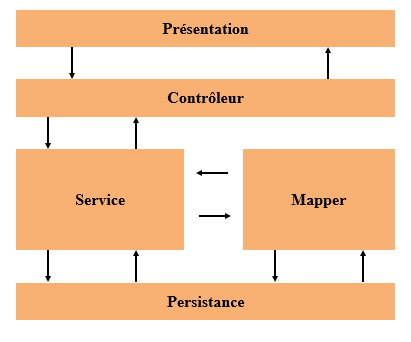
\includegraphics[scale=1]{img/archi logique.PNG}
     \caption{Architecture logique du module de gestion des candidats}
     \label{fig:archi_logique}
 \end{figure}
 %%%%%%%%%%%%%%%%%%%%%%%%%%%%%%%%%%%%%%%%%%%%%%%%%%%
 \subsection{Diagramme de paquetage}
 Notre application doit garantir une indépendance dans les rôles entre ses différents modules qui sont représentés dans la Figure \ref{fig:diagram_package} :
 \begin{itemize}
     \item Le paquetage \textbf{Controller} contient les web services REST.
     \item Le paquetage \textbf{Dto} contient les différentes classes Dto qui représentent les objets envoyés et reçus de la partie frontend.
     \item Le paquetage \textbf{Services} contient les différentes classes de la logique métier.
     \item Le paquetage \textbf{Mapper} contient les différentes classes qui permettent la transformation des objets Dto en des entités pour les enregistrer, les modifier ou les supprimer de la base de données.
     \item Le paquetage \textbf{Dao} contient les différentes interfaces contenant les méthodes qui permettent la persistance des données dans la base de données.
     \item Le paquetage \textbf{Entities} contient les différentes classes des entités relatives aux tables de la base de données.
 \end{itemize}
  \begin{figure}[H]
     \centering
     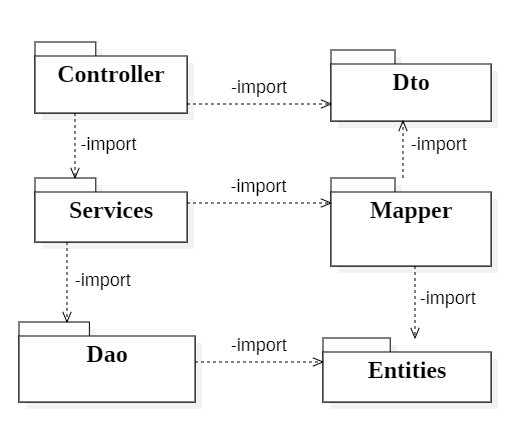
\includegraphics[scale=0.8]{img/Package Diagram.png}
     \caption{Diagramme de paquetage}
     \label{fig:diagram_package}
 \end{figure}
 %%%%%%%%%%%%%%%%%%%%%%%%%%%%%%%%%%%%%%%%%%%%%%%%%%%
\section{Conception détaillée}
Après avoir précisé les différents aspects de la conception générale de notre application, nous passons à la conception détaillée. Dans cette section, nous présentons le diagramme de classe ainsi que les diagrammes de séquences.
\subsection{Diagramme de classes}
Les diagrammes de classes sont l'un des types de diagrammes les plus utiles, car ils décrivent clairement la structure d’un système particulier en modélisant ses classes, ses attributs, ses opérations et les relations entre ses objets. La Figure \ref{fig:diagram_class} représente le diagramme de classes relatif à notre application.
 \begin{figure}[H]
     \centering
     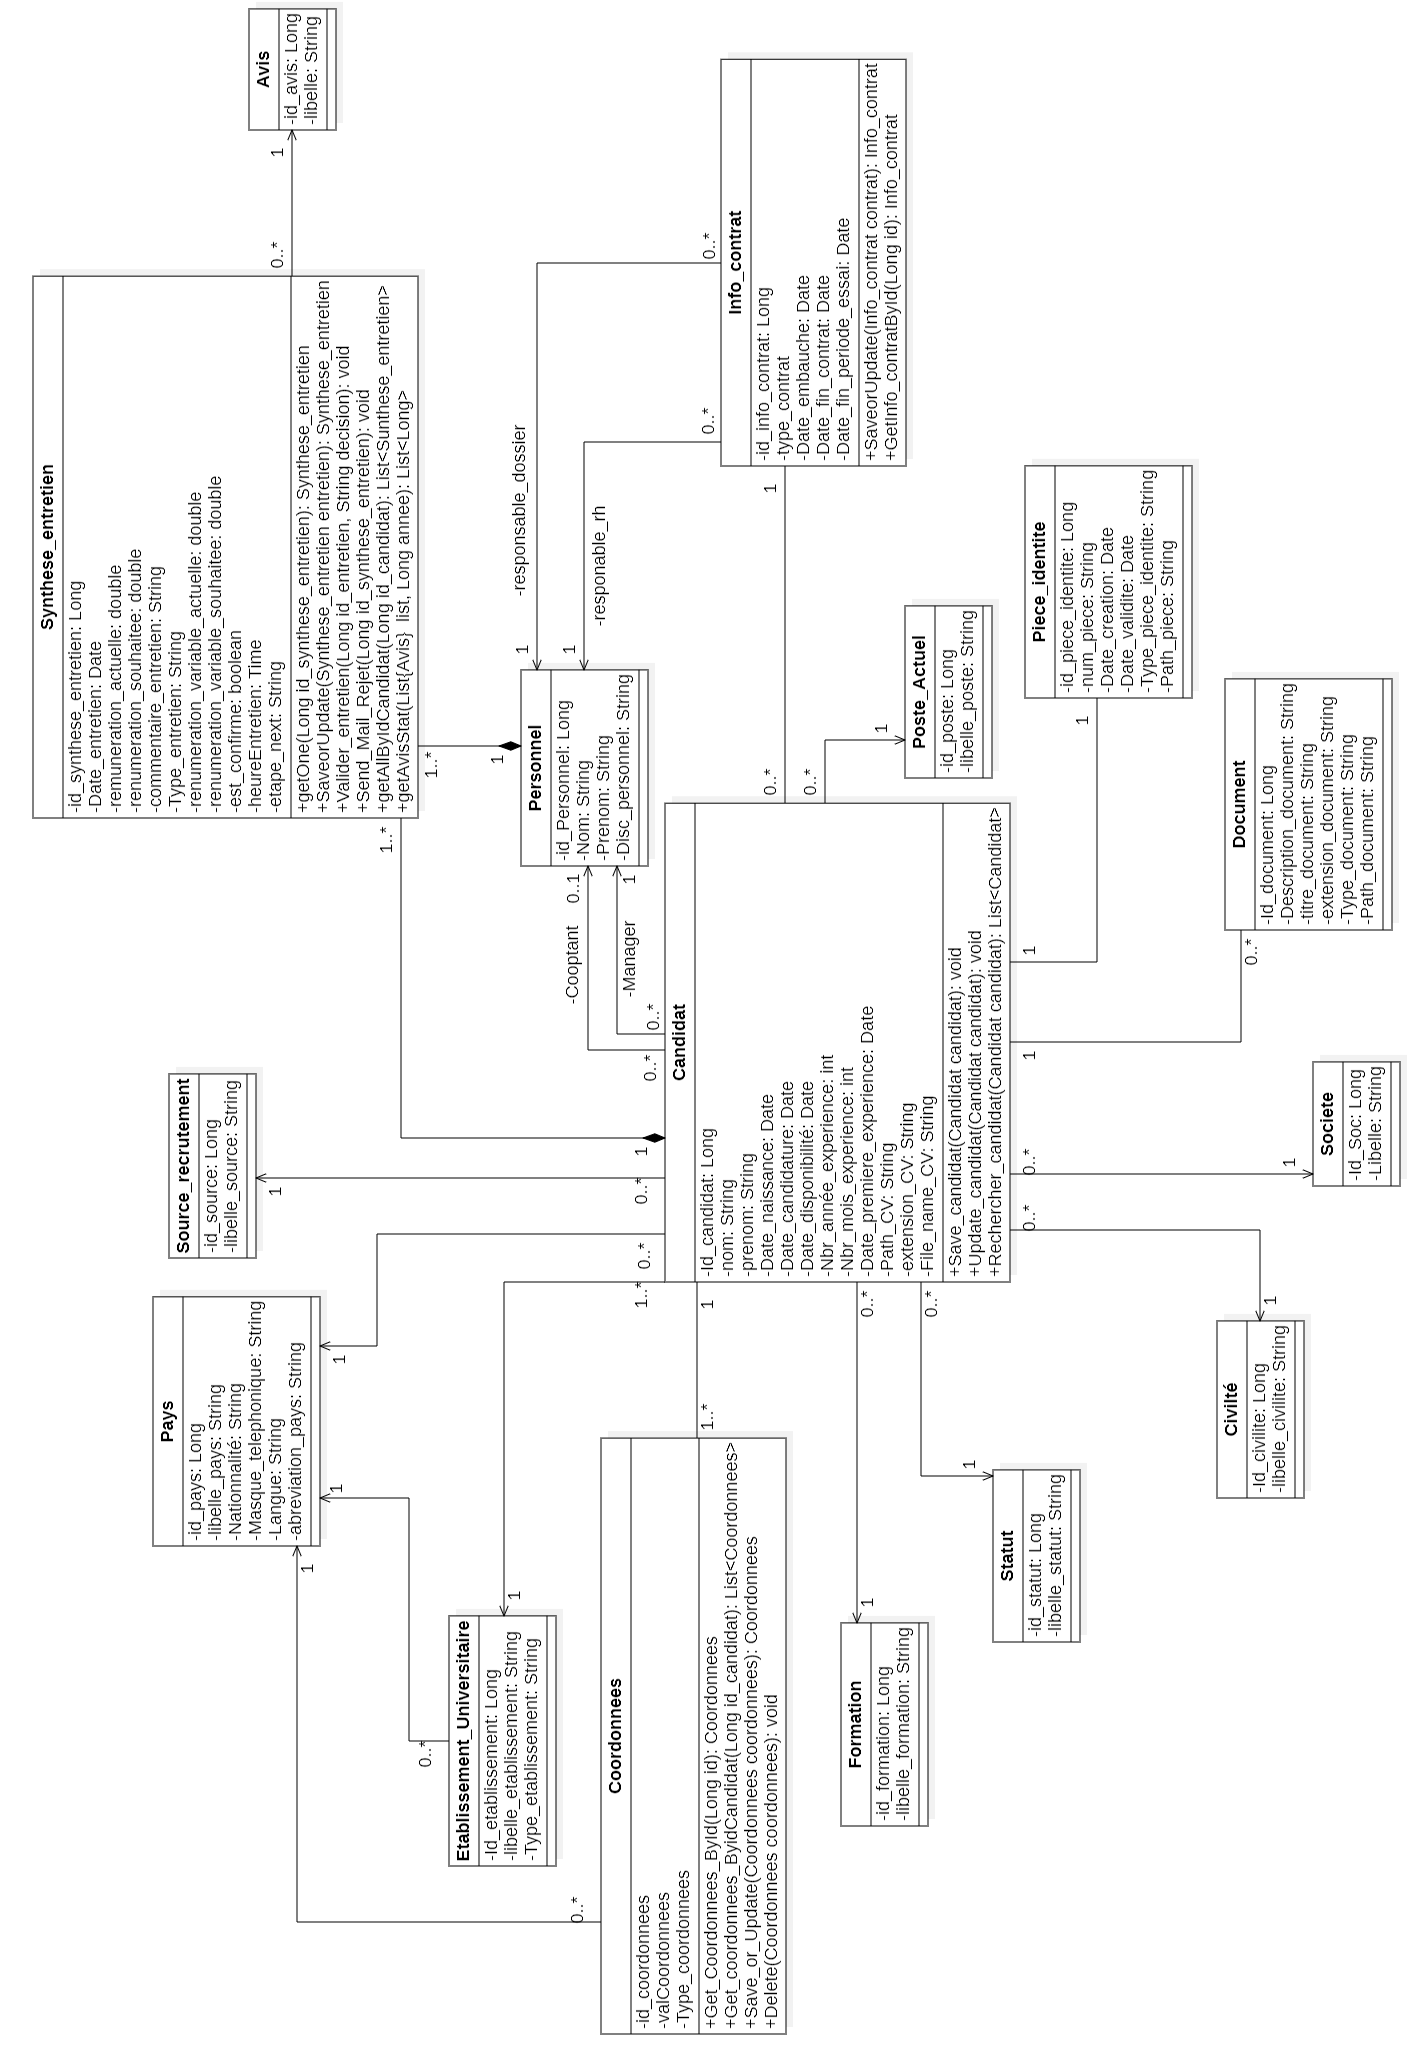
\includegraphics[scale=0.45]{img/ClassDiagram2.png}
     \caption{Diagramme de classes}
     \label{fig:diagram_class}
 \end{figure}
\newpage
Le diagramme représenté par la Figure \ref{fig:diagram_class} est constitué des classes suivantes:
\begin{itemize}
    \item \textbf{Classe coordonnées} : cette classe permet de gérer les coordonnées relatives à un candidat (un e-mail ou bien un numéro de téléphone).
    \item \textbf{Classe Info\_contrat} : cette classe permet de gérer les informations concernant le contrat (salaire, durée,poste, régime\dots) à signer par candidat s'il sera accepté.
    \item \textbf{Classe Synthese\_entretien} : cette classe permet de gérer les entretiens du candidat.
    \item \textbf{ Classe Candidat} : cette classe permet de gérer la fiche du candidat.
    
\end{itemize}
\subsection{Diagrammes de séquences}
Les diagrammes de séquences sont la représentation graphique des interactions entre les acteurs et le système selon un ordre chronologique. Dans cette partie, nous présentons les principaux diagrammes de séquences relatifs aux fonctionnalités de notre application.
\subsubsection{Ajouter une fiche candidat}
La Figure \ref{fig:sequence_ajout_fiche} représente le diagramme de séquence relatif à l'ajout d'une nouvelle fiche candidat. 
 \begin{figure}[H]
     \centering
     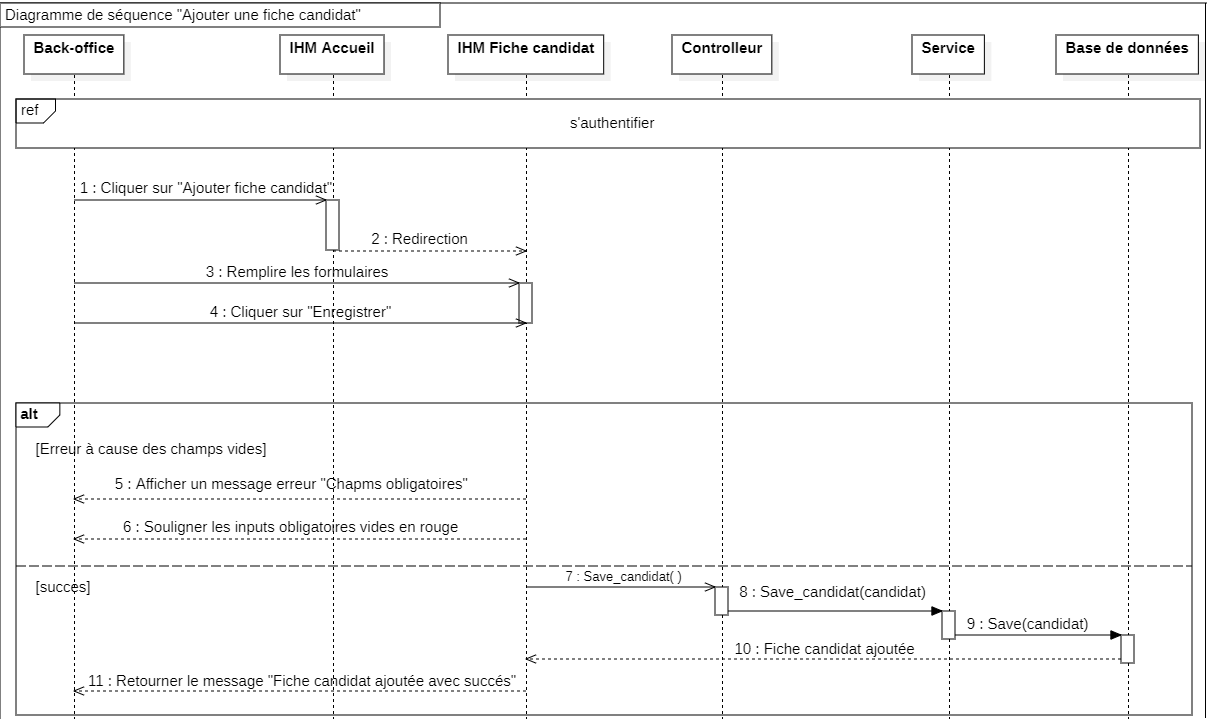
\includegraphics[scale=0.51]{img/sequence ajouter fiche candidat.png}
     \caption{Diagramme de séquence "Ajouter une fiche candidat"}
     \label{fig:sequence_ajout_fiche}
 \end{figure}
 Le back-office doit s'authentifier pour accéder à l'interface de la fiche candidat en cliquant sur "Ajouter fiche candidat" à partir de l'interface d'accueil. Il doit ensuite remplir le formulaire de la fiche et cliquer sur "Enregistrer". Un objet candidat est envoyé au contrôleur qui le passe, à son tour, au service pour l'enregistrer dans la base de données.
 %%%%%%%%%%%%%%%%%%%%%%%%%%%%%%%%%%%%%%%%%%%%%
 \subsubsection{Rechercher un candidat}
 Le diagramme de séquence du cas d'utilisation "Rechercher un candidat" est représenté par la Figure \ref{fig:sequence_recherche_candidat}
  \begin{figure}[H]
     \centering
     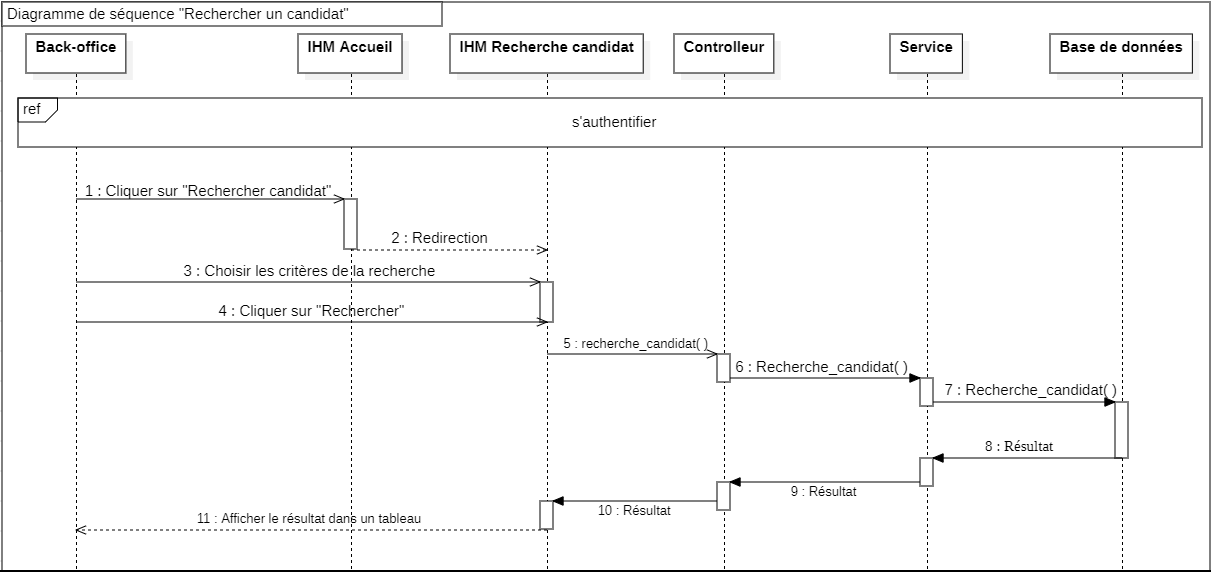
\includegraphics[scale=0.51]{img/sequence recherche candidat.png}
     \caption{Diagramme de séquence "Rechercher un candidat"}
     \label{fig:sequence_recherche_candidat}
 \end{figure}
 Après authentification, le back-office clique sur le bouton "Rechercher un candidat". Une fois l'interface de la recherche est chargée, le back-office choisit les critères de recherche(liste déroulante,case à cocher$\dots$) et clique sur le bouton "Rechercher". Un objet contenant les critères de recherche est envoyé au contrôleur, puis passé au service afin d'exécuter la méthode de la recherche. Le résultat est envoyé sous forme d'une liste des candidats à l'interface de la recherche où le résultat est affiché sous forme d'un tableau. Chaque ligne du tableau contient quelques informations qui concernent le candidat ainsi qu'un bouton pour consulter la fiche du candidat. 
 %\newpage
 %%%%%%%%%%%%%%%%%%%%%%%%%%%%%%%%%%%%%%%%%%%%%%%%%
 \subsubsection{Planifier un entretien}
 La Figure \ref{fig:sequence_planifier_entretien} illustre le diagramme de séquence relatif à la planification d'un nouvel entretien.
 \newpage
 \begin{figure}[H]
     \centering
     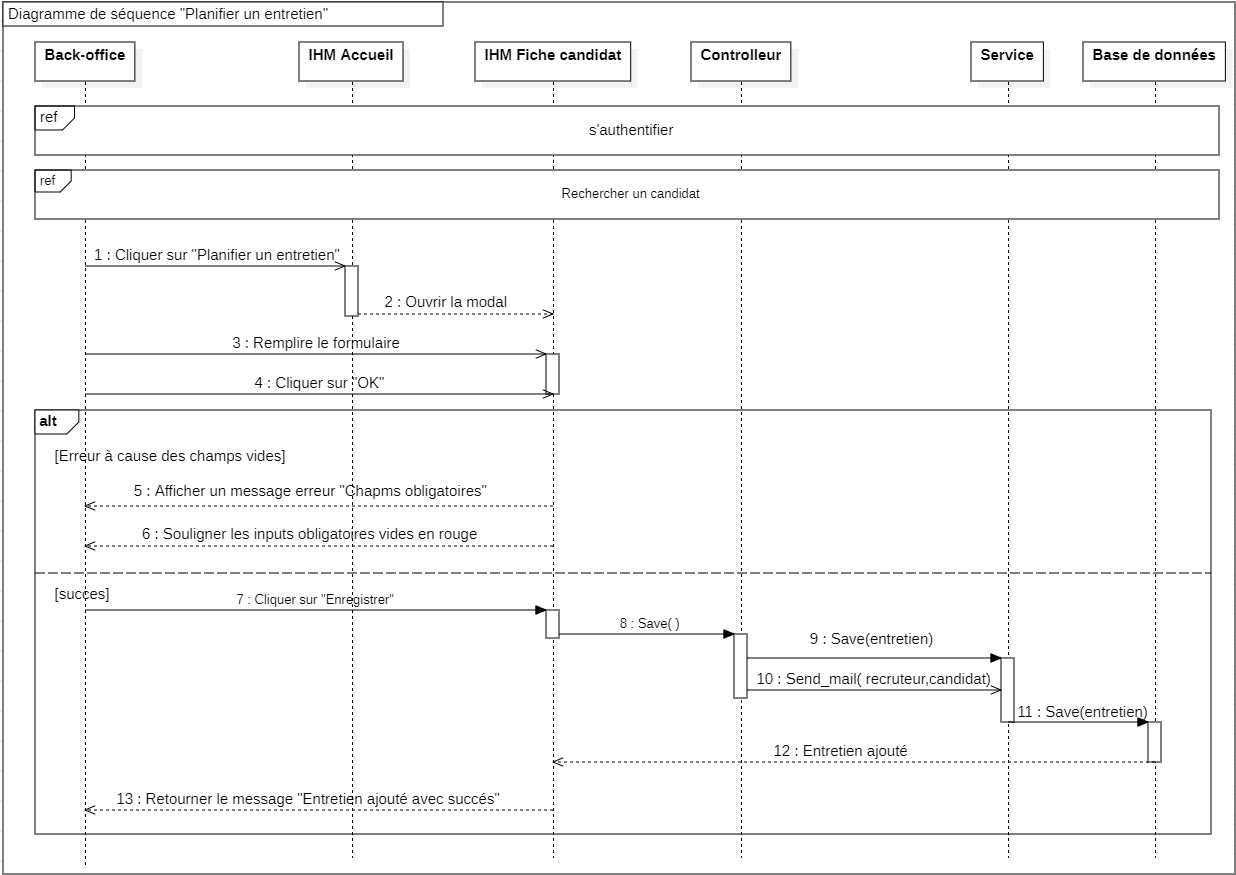
\includegraphics[scale=0.51]{img/sequence planifier entretien.png}
     \caption{Diagramme de séquence "Planifier un entretien"}
     \label{fig:sequence_planifier_entretien}
 \end{figure}
 Une fois le back-office s'est authentifié et a effectué une recherche, il planifie un nouvel entretien en cliquant sur le bouton "Planifier un entretien". Après, il remplit le formulaire et clique sur "OK". Le système vérifie qu'il n'y a pas des champs obligatoires vides et enregistre l'entretien. Enfin, un e-mail est envoyé pour  notifier le recruteur sélectionné lors de la planification de l'entretien.
 %%%%%%%%%%%%%%%%%%%%%%%%%%%%%%%%%%%%%%%%%%%%%%%%%
 \subsubsection{Accepter un entretien}
 Le diagramme de séquence relatif au cas d'utilisation "Accepter un entretien" est représenté dans la Figure \ref{fig:sequence_accepter_entretien}.
 \begin{figure}[H]
     \centering
     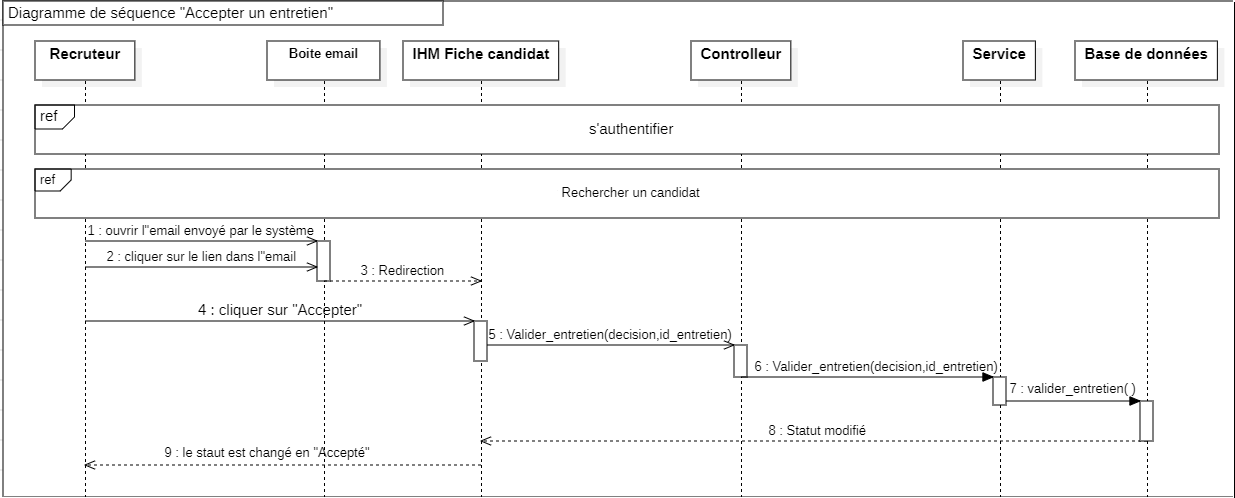
\includegraphics[scale=0.51]{img/sequence accepter entretien.png}
     \caption{Diagramme de séquence "Accepter un entretien"}
     \label{fig:sequence_accepter_entretien}
 \end{figure}
 Une fois un entretien est planifié, le recruteur consulte l'e-mail reçu dans son courrier électronique et contenant les informations relatives à l'entretien. Il clique alors sur le lien qui lui est envoyé dans l'e-mail et qui le redirige vers la fiche du candidat. Il clique sur le bouton "Accepter", ce qui modifie le statut de l'entretien en "Accepté".
 %%%%%%%%%%%%%%%%%%%%%%%%%%%%%%%%%%%%%%%%%%%%%%%%%%%
 \subsubsection{Rejeter un entretien}
 La Figure \ref{fig:sequence_refuser_entretien} représente le diagramme de séquence relatif au cas d'utilisation "Rejeter un entretien".
 \begin{figure}[H]
     \centering
     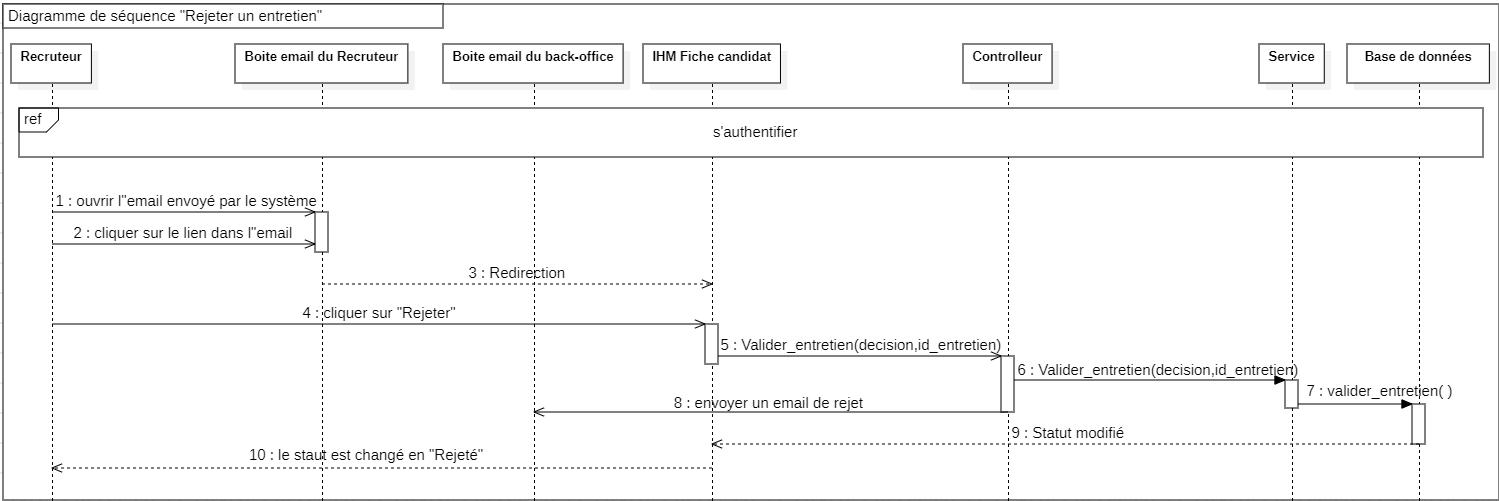
\includegraphics[scale=0.4]{img/sequence refuser entretien.png}
     \caption{Diagramme de séquence "Rejeter un entretien"}
     \label{fig:sequence_refuser_entretien}
 \end{figure}
   Une fois un entretien est planifié, le recruteur consulte l'e-mail reçu dans son courrier électronique et contenant les informations relatives à l'entretien. Il clique alors sur le lien qui lui est envoyé dans l'e-mail et qui le redirige vers la fiche du candidat. Il clique sur le bouton "Rejeter", un e-mail est alors envoyé au back-office pour le notifier du rejet de l'entretien par le recruteur. Ainsi, le statut de l'entretien est modifié en "Rejeté".
  %%%%%%%%%%%%%%%%%%%%%%%%%%%%%%%%%%%%%%%%%%%%%%%%%%%%
 \subsubsection{Modifier une fiche candidat}
 Le diagramme de séquence relatif à la modification d'une fiche candidat est représenté dans la Figure \ref{fig:sequence_modif_fiche}.
 \begin{figure}[H]
 \centering
 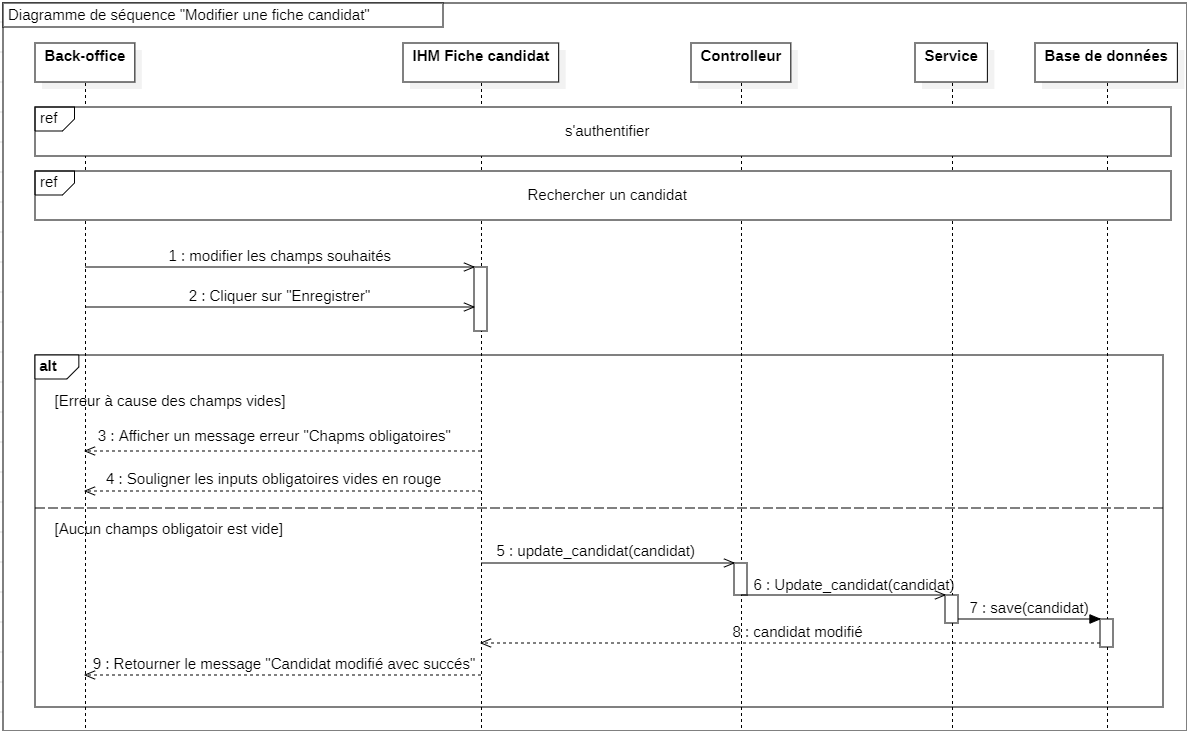
\includegraphics[scale=0.51]{img/sequence modifier fiche candidat.png}
 \caption{Diagramme de séquence "Modifier une fiche candidat"}
 \label{fig:sequence_modif_fiche}
 \end{figure}
 Après son authentification, et la recherche de la fiche d'un candidat, le back-office procède au modifications de champs qu'il juge nécessaires dans le formulaire affiché, puis clique sur le bouton "Enregistrer". Le système vérifie que les champs obligatoires sont remplis et enregistre les modifications. Enfin, un message contenant "Candidat modifié avec succès" est affiché.
 %%%%%%%%%%%%%%%%%%%%%%%%%%%%%%%%%%%%%%%%%%%%%%%%%%%%%%
\section*{Conclusion}
Dans le présent chapitre, nous avons présenté la conception générale de notre application. Par la suite, nous avons passé en revue la conception détaillée, en enchaînant par le diagramme de classes ainsi que les diagrammes de séquences pour mieux visualiser l'interaction des acteurs avec le système.
Dans le prochain chapitre, nous allons montrer comment nous avons traduit cette étude conceptuelle et à l’aide de quels outils nous avons pu mettre en place notre application.

        \clearpage
        
        \chapter{Réalisation}
%%%%%%%%%%%%%%%%%%%%%%%%%%%%%%%%%%%%%%%%%%%%%%%%%
\section*{Introduction}
Tenant compte des besoins fixés et des choix conceptuels effectués, nous consacrons
ce chapitre à l’exposition du travail réalisé. Nous commençons par la description de
l’environnement matériel et logiciel utilisés. Nous terminons par des captures d’écrans traduisant le déroulement du projet et présentant les fonctionnalités développées.
%Pour finaliser notre projet, nous entamons la partie réalisation qui présente une importance, tant pour nous que pour la société concernée. Nous commençons par argumenter les choix matériel et logiciel, en présentant l’architecture du système ainsi que les technologies utilisées pour l’implémentation. Enfin, nous passons à la présentation de l’application par l’élaboration des captures d’écrans produites.
%%%%%%%%%%%%%%%%%%%%%%%%%%%%%%%%%%%%%%%%%%%%%%%%%
\section{Environnement de travail}
Dans ce paragraphe, nous présentons les outils matériels et logiciels adoptés pour l’achèvement de notre projet.
\subsection{Environnement matériel}
Notre application a été réalisée sur un ordinateur ayant les caractéristiques suivantes : 
\begin{itemize}
    \item Un processeur Intel(R) Core(TM) i5-5200U CPU @ 2.20GHz 2.20 GHz.
    \item Une mémoire RAM de 12 Go.
    \item Un disque dur de 1 To.
    \item Un système d'exploitation Windows 10.
\end{itemize}
%%%%%%%%%%%%%%%%%%%%%%%%%%%%%%%%%%%%%%%%%%%%%%%%%
\subsection{Environnement logiciel}
Dans cette partie, nous présentons les différents logiciels et outils utilisés:
\begin{itemize}
    \item \textbf{StarUML} \\
    C'est un logiciel de modélisation UML qui gère la plupart des diagrammes spécifiés dans la norme UML 2.0.
    \item \textbf{PostgreSQL}\\
    C'est un puissant système de gestion de bases de données open source. PostgreSQL fonctionne sur tous les principaux systèmes d'exploitation.
    \item \textbf{Intellij IDEA}\\
    C'est un environnement de développement intégré de technologie Java. Il est destiné au développement de logiciels informatiques.
    \item \textbf{Visual Studio Code}\\
    C'est un éditeur de code source, léger mais puissant. Il dispose d'un riche écosystème d'extensions pour d'autres langages (tels que C ++, C\#, Java, Python, PHP, Go).
    \item \textbf{Docker}\\
    C'est un logiciel libre permettant de lancer des applications dans des conteneurs logiciels. Un conteneur est une unité logicielle standard qui regroupe le code et toutes ses dépendances, et qui permet à l'application de s'exécuter rapidement et de manière fiable, d'un environnement informatique à un autre.
    \item \textbf{Overleaf}\\
    C'est un éditeur LaTeX en ligne, collaboratif en temps réel. Il est utilisé pour la rédaction, l'édition et la publication de documents scientifiques.
\end{itemize}
%%%%%%%%%%%%%%%%%%%%%%%%%%%%%%%%%%%%%%%%%%%%%%%%%
\subsection{Technologies utilisées}
Dans cette partie, nous nous intéressons aux langages et aux bibliothèques utilisés tout au long de la réalisation de notre application tout en justifiant notre choix.
\begin{itemize}
    \item \textbf{Spring Boot}\\
    C'est un framework de développement applicatif JAVA open Source. Il est particulièrement recommandé pour le développement des microservices. Ses points forts sont l'auto-configuration ainsi que les annotations.
    \item \textbf{Spring Cloud Eureka Client}\\
    Il permet aux différents microservices de s'enregistrer dans l'annuaire des services Eureka. La Figure \ref{fig:capture_eureka} montre la liste des microservices détectés par le service Eureka. 
    \begin{figure}[H]
     \centering
     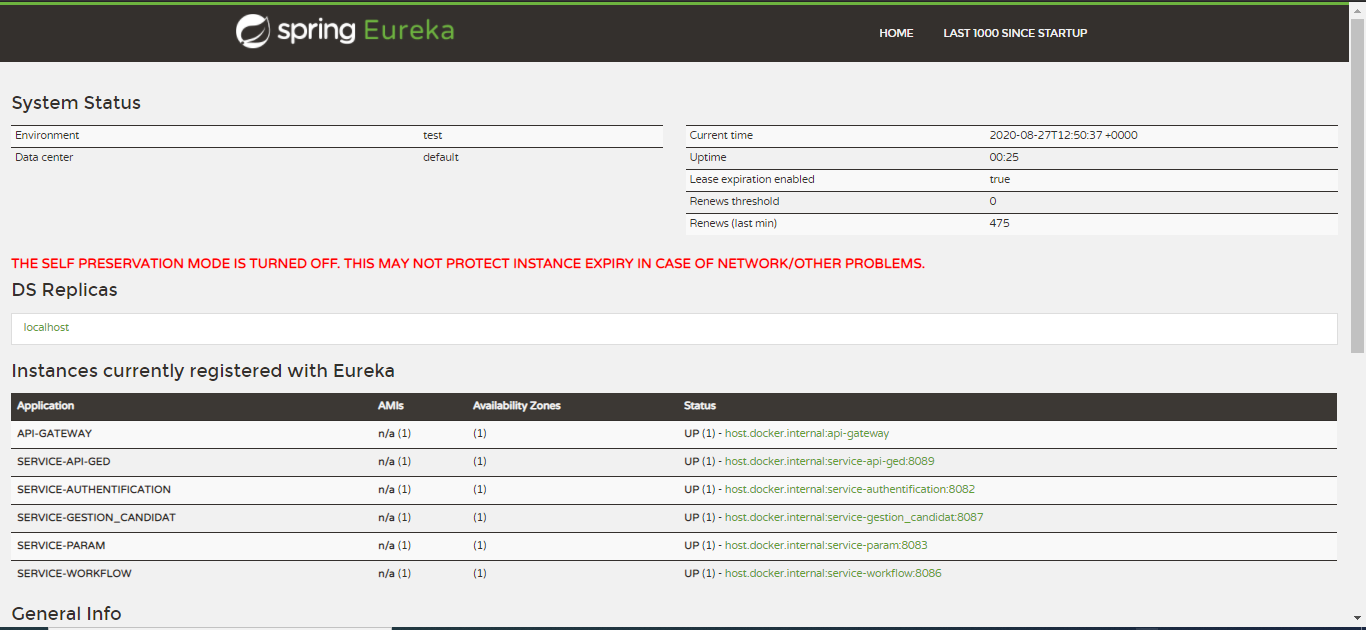
\includegraphics[scale=0.47]{img/capture eureka.PNG}
     \caption{Interface de Eureka Discovery Service}
     \label{fig:capture_eureka}
 \end{figure}
    \item \textbf{Spring Data JPA}\\
    Il vise à améliorer d'une manière significative la mise en oeuvre des couches d'accès aux données en réduisant la quantité de code à écrire.
    \item \textbf{QueryDsl}\\
    C'est un framework qui permet la construction des requêtes SQL typées dynamiquement via son API fluide.
    \item \textbf{Angular 7}\\
    C'est framework JavaScript libre, développé par Google et utilisé pour créer des applications Web basées sur une seule page (Single Page Application). Il utilise des fonctionnalités de plate-forme Web modernes pour offrir de nouvelles expériences, ayant une installation à haute performance avec zéro-étape.
\end{itemize}
%%%%%%%%%%%%%%%%%%%%%%%%%%%%%%%%%%%%%%%%%%%%%%%%%
\section{Les interfaces utilisateur}
Nous exposerons dans cette section les interfaces homme-machine qui sont un élément important pour la réussite d'une application.
%%%%%%%%%%%%%%%%%%%%%%%%%%%%%%%%%%%%%%%%%%%%%%%%%
\subsection{Interface d'authentification}
Pour pouvoir accéder aux différentes fonctionnalités de l’application, l'utilisateur doit saisir son login et son mot de passe comme le montre la Figure \ref{fig:capture_auth}.
\begin{figure}[H]
     \centering
     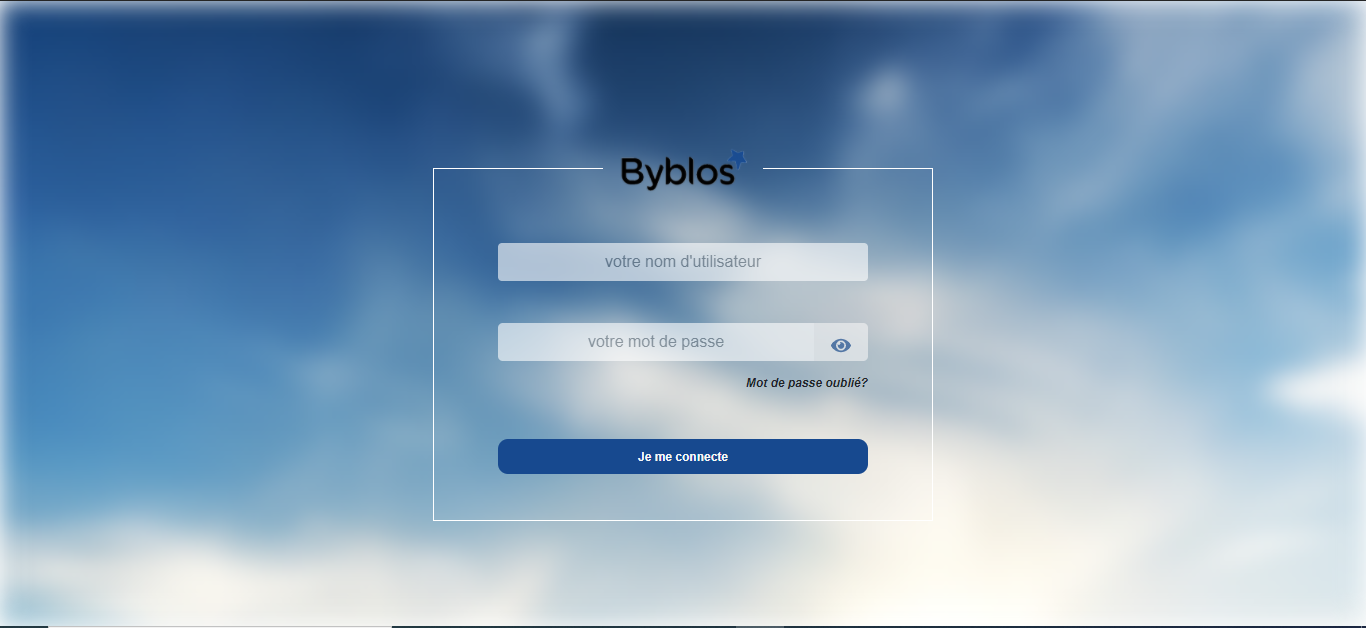
\includegraphics[scale=0.5]{img/capture authentification.PNG}
     \caption{Interface d'authentification}
     \label{fig:capture_auth}
 \end{figure}
%%%%%%%%%%%%%%%%%%%%%%%%%%%%%%%%%%%%%%%%%%%%%%%%%%%
\subsection{Interface d'accueil}
Après l'authentification de l'utilisateur, la page d'accueil est chargée comme le montre la Figure \ref{fig:capture_accueil}. Elle contient le KPI des avis des entretiens composé des éléments suivants :
\begin{itemize}
    \item Une liste prédéfinie des avis distingués par des couleurs différentes.
    \item Un graphe en secteurs de différentes couleurs. Chaque secteur contient le nombre total de candidats correspondant à un avis donné.
    \item L'année choisie ainsi que deux boutons pour sélectionner l'année suivante ou bien l'année précédente.
    \item Deux boutons en bas, l'un dirige vers une nouvelle fiche candidat, l'autre vers l'interface de recherche de candidats.  
    
\end{itemize}
 
\begin{figure}[H]
     \centering
     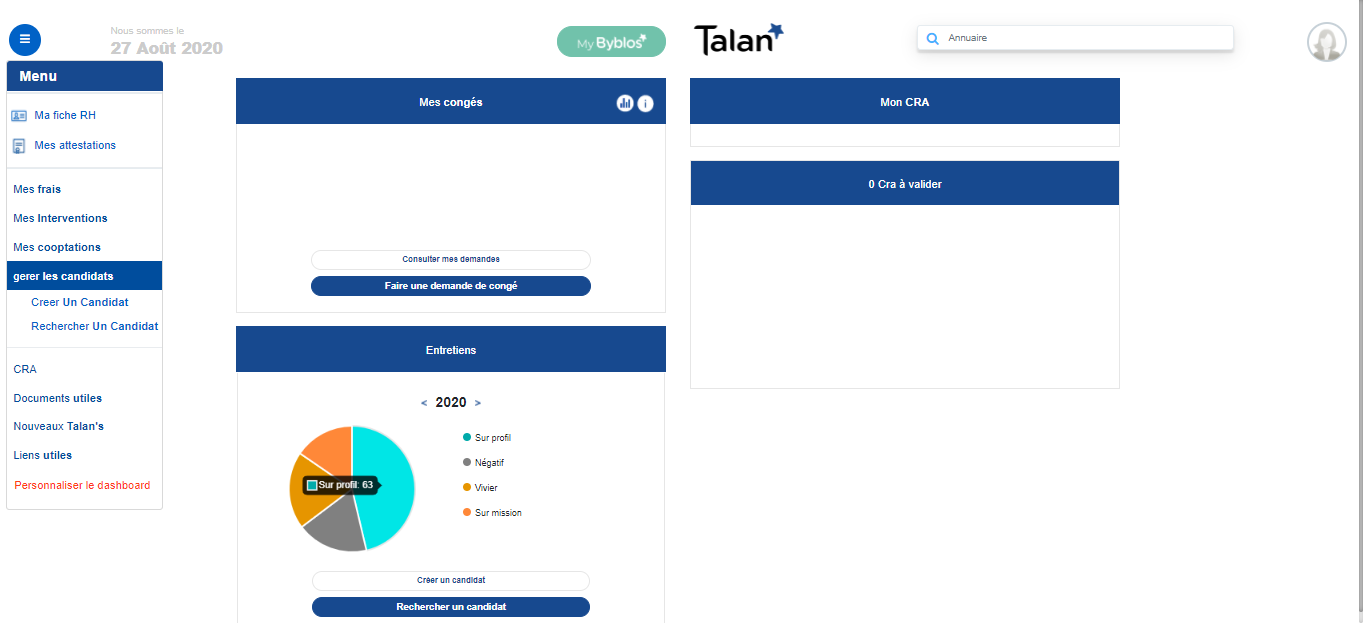
\includegraphics[scale=0.5]{img/capture accueil 2.png}
     \caption{Interface d'accueil}
     \label{fig:capture_accueil}
 \end{figure}
%%%%%%%%%%%%%%%%%%%%%%%%%%%%%%%%%%%%%%%%%%%%%%%%%%%
\subsection{Interface d'ajout d'une fiche candidat}
Cette interface est composée de trois parties :
\begin{enumerate}[label=\textbf{\arabic*. }]
    \item \textbf{Fiche candidat} : elle contient les informations qui concernent le candidat. Cette partie se compose de quatre formulaires listés ci-dessous :
    \begin{enumerate}
        \item [•] \textbf{Interface identité:} \\Cette interface, représentée dans la Figure \ref{fig:capture_fiche_identité}, contient les informations liées à l'identité du candidat: son nom, son prénom, sa date de naissance $\dots$ 
         \begin{figure}[H]
     \centering
     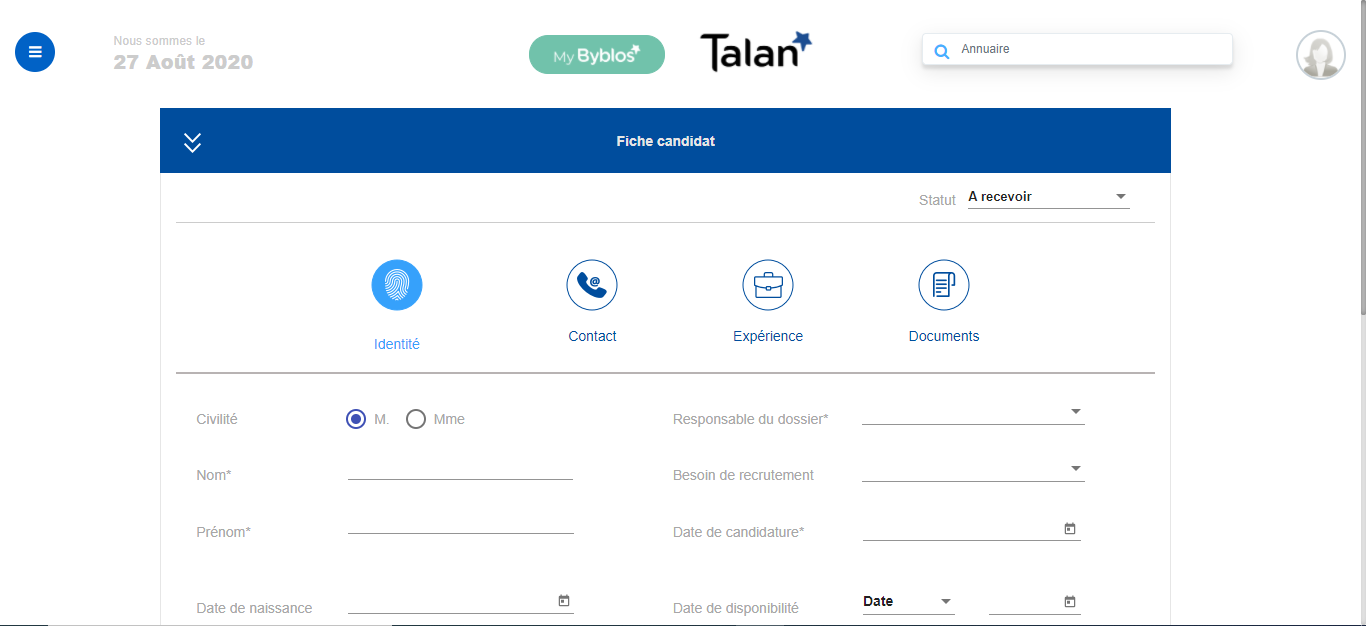
\includegraphics[scale=0.5]{img/capture fiche candidat identite.PNG}
     \caption{Interface Identité}
     \label{fig:capture_fiche_identité}
 \end{figure}
    \end{enumerate}
    \item [•] \textbf{Interface contact:}\\Cette interface, représentée dans la Figure \ref{fig:capture_fiche_contact}, contient les coordonnées du candidat: son numéro du téléphone et son e-mail.
    \begin{figure}[H]
     \centering
     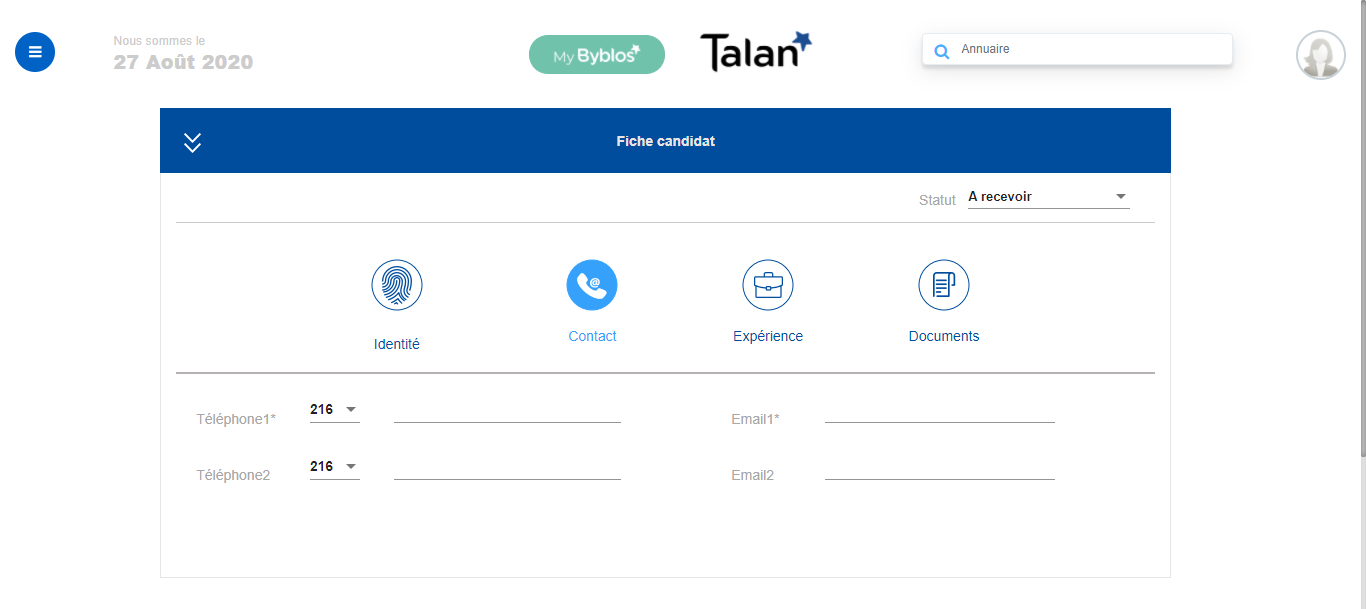
\includegraphics[scale=0.5]{img/capture fiche candidat contact.PNG}
     \caption{Interface Contact}
     \label{fig:capture_fiche_contact}
 \end{figure}
    \item [•] \textbf{Interface expérience:}\\ Cette interface, représentée dans la Figure \ref{fig:capture_fiche_experience}, contient les informations concernant l'expérience professionnelle du candidat.  
     \begin{figure}[H]
     \centering
     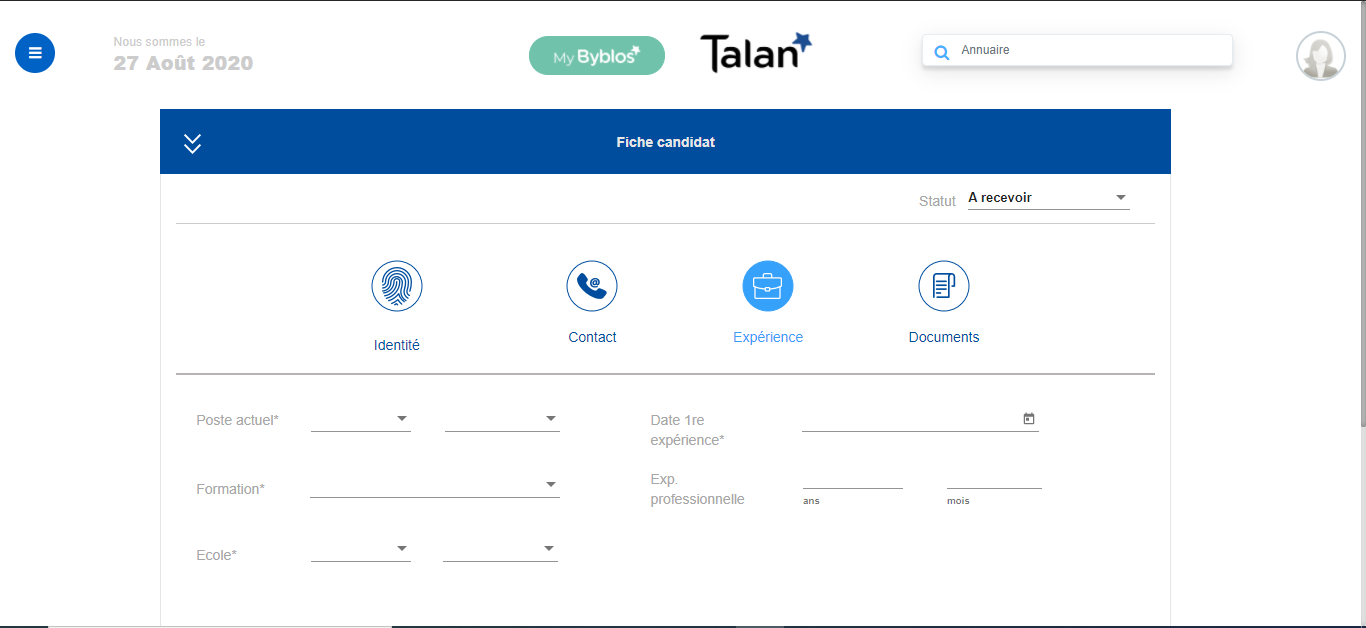
\includegraphics[scale=0.5]{img/capture fiche candidat experience.PNG}
     \caption{Interface Expérience}
     \label{fig:capture_fiche_experience}
 \end{figure}
    \item [•] \textbf{Interface Documents:}\\ Cette interface, représentée dans la Figure \ref{fig:capture_fiche_documents}, contient les informations concernant la pièce d'identité du candidat ainsi que son CV.
     \begin{figure}[H]
     \centering
     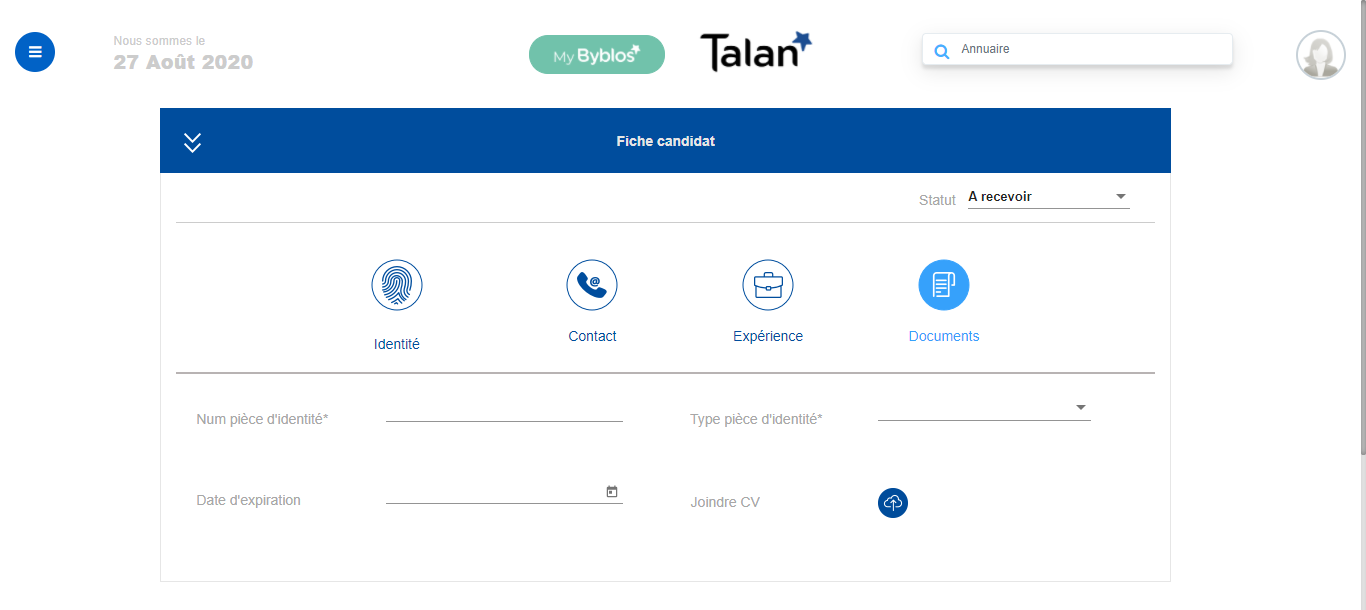
\includegraphics[scale=0.5]{img/capture fiche candidat Documents.PNG}
     \caption{Interface Documents}
     \label{fig:capture_fiche_documents}
 \end{figure}
\item \textbf{Planification des entretiens:}\\ Cette interface, représentée dans la Figure \ref{fig:capture_planifier_entretiens}, contient la liste des entretiens déjà planifiés, avec un bouton permettant de planifier un nouvel entretien.
 \begin{figure}[H]
     \centering
     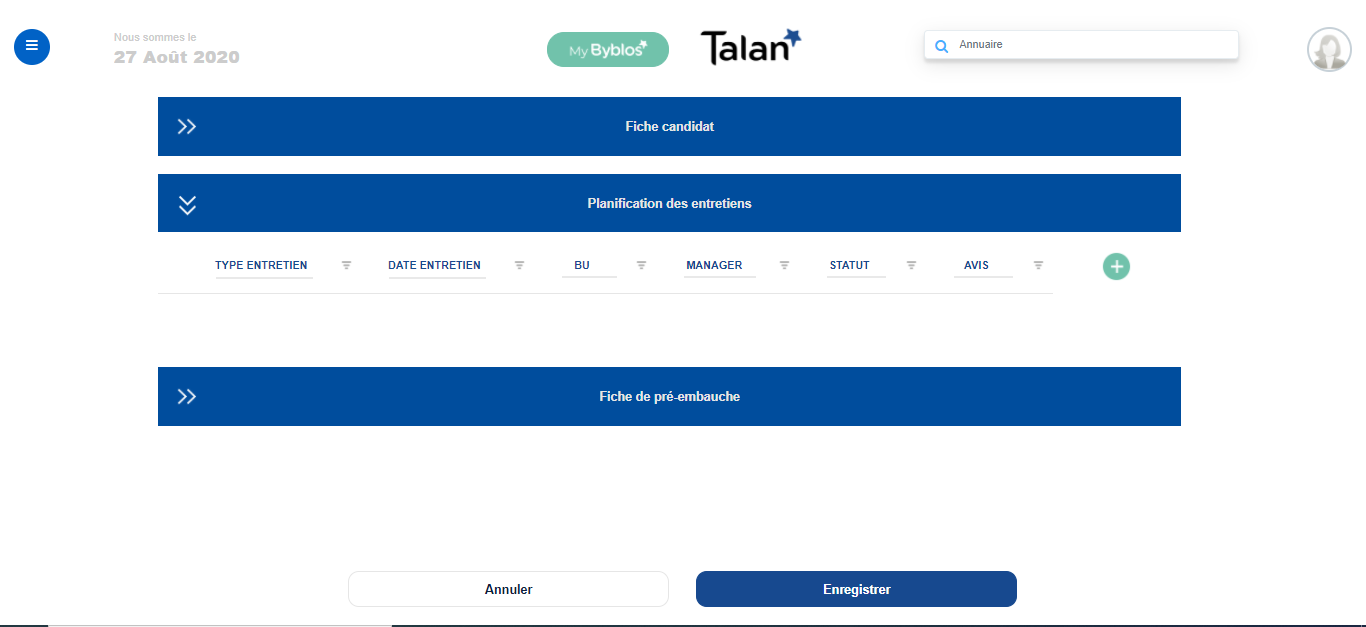
\includegraphics[scale=0.5]{img/capture fiche candidat 1.PNG}
     \caption{Interface Planification des entretiens}
     \label{fig:capture_planifier_entretiens}
 \end{figure}
\item \textbf{Fiche de pré-embauche}\\ Cette interface contient les informations concernant le contrat de pré-embauche à signer par le candidat s'il est accepté. Cette interface est composée de trois formulaires listés ci-dessous :
\begin{enumerate}
    \item [•] \textbf{Interface contrat} \\ Cette interface, représentée dans la Figure \ref{fig:capture_embauche_contrat}, contient les différentes informations contenues dans le contrat à signer.
    \begin{figure}[H]
     \centering
     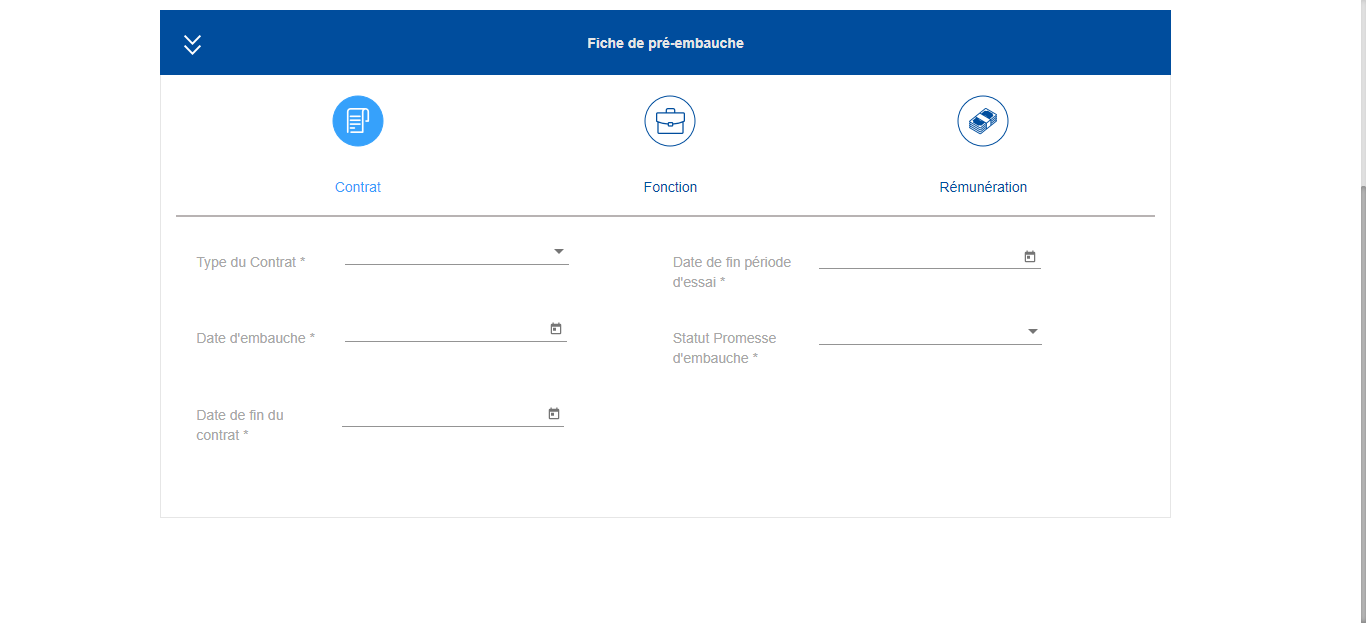
\includegraphics[scale=0.5]{img/capture fiche pre-embauche contrat.PNG}
     \caption{Interface Contrat}
     \label{fig:capture_embauche_contrat}
 \end{figure}
    \item [•] \textbf{Interface fonction} \\  Cette interface, représentée dans la Figure \ref{fig:capture_embauche_fonction}, contient les informations concernant la fonction que le candidat va occuper.
    \begin{figure}[H]
     \centering
     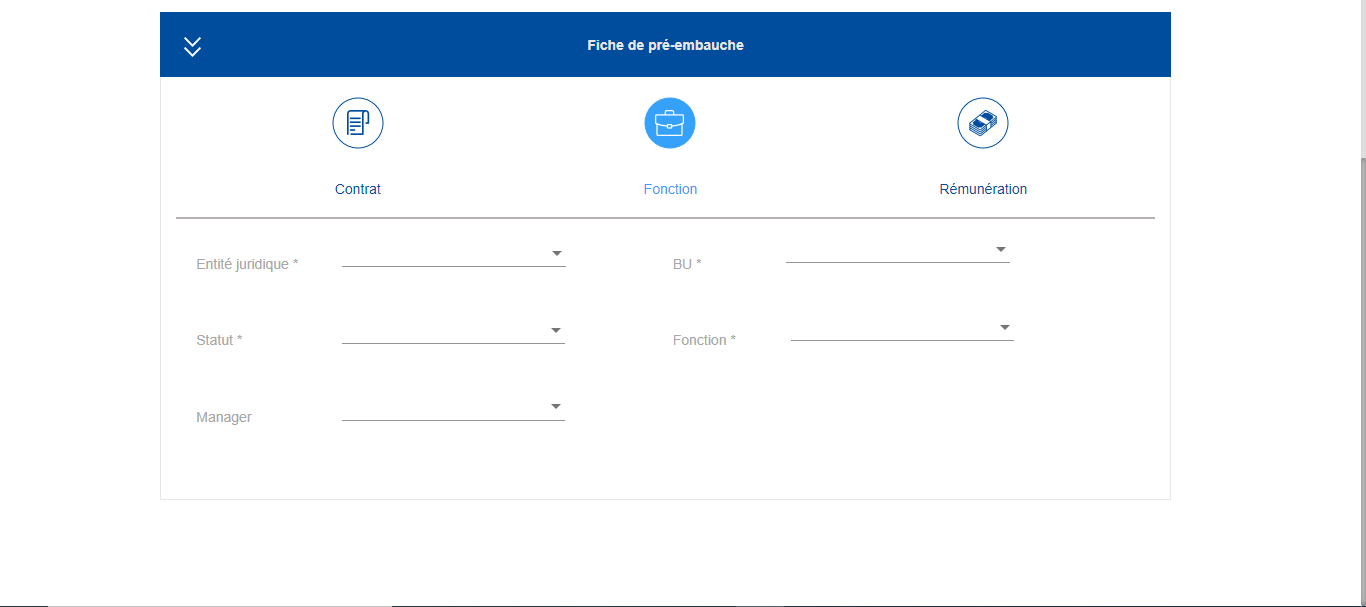
\includegraphics[scale=0.5]{img/capture fiche pre-embauche fonction.PNG}
     \caption{Interface Fonction}
     \label{fig:capture_embauche_fonction}
 \end{figure}
    \item [•] \textbf{Interface rémunération} \\ Cette interface, représentée dans la Figure \ref{fig:capture_embauche_remuneration}, contient les informations concernant la rémunération qui sera attribuée au candidat. 
    \begin{figure}[H]
     \centering
     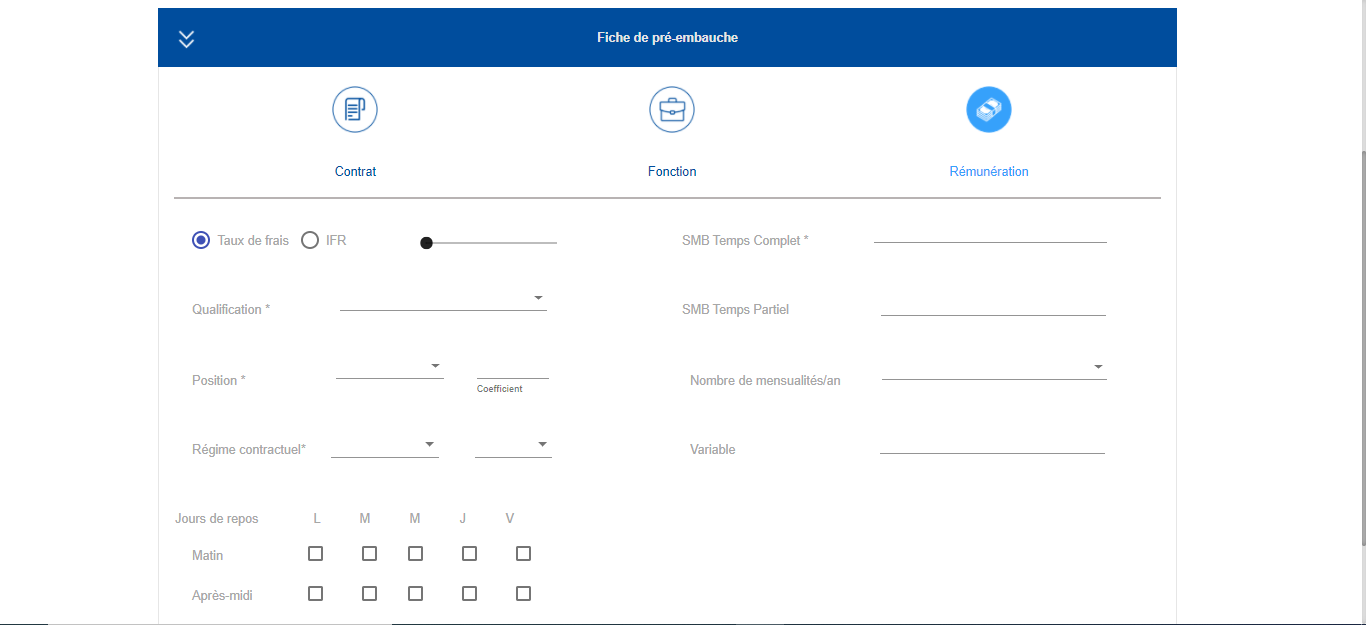
\includegraphics[scale=0.5]{img/capture fiche pre-embauche remuneration.PNG}
     \caption{Interface Rémunération}
     \label{fig:capture_embauche_remuneration}
 \end{figure}
\end{enumerate}
\end{enumerate}
%%%%%%%%%%%%%%%%%%%%%%%%%%%%%%%%%%%%%%%%%%%%%%%%%
\subsection{Interface de la recherche d'un candidat}
Cette interface, représentée dans la Figure \ref{fig:capture_recherche}, comporte un filtre contenant les critères de recherche sélectionnés, avec la possibilité d'omettre certains d'entre eux ainsi que le formulaire de recherche et un tableau contenant le résultat obtenu.
\begin{figure}[H]
     \centering
     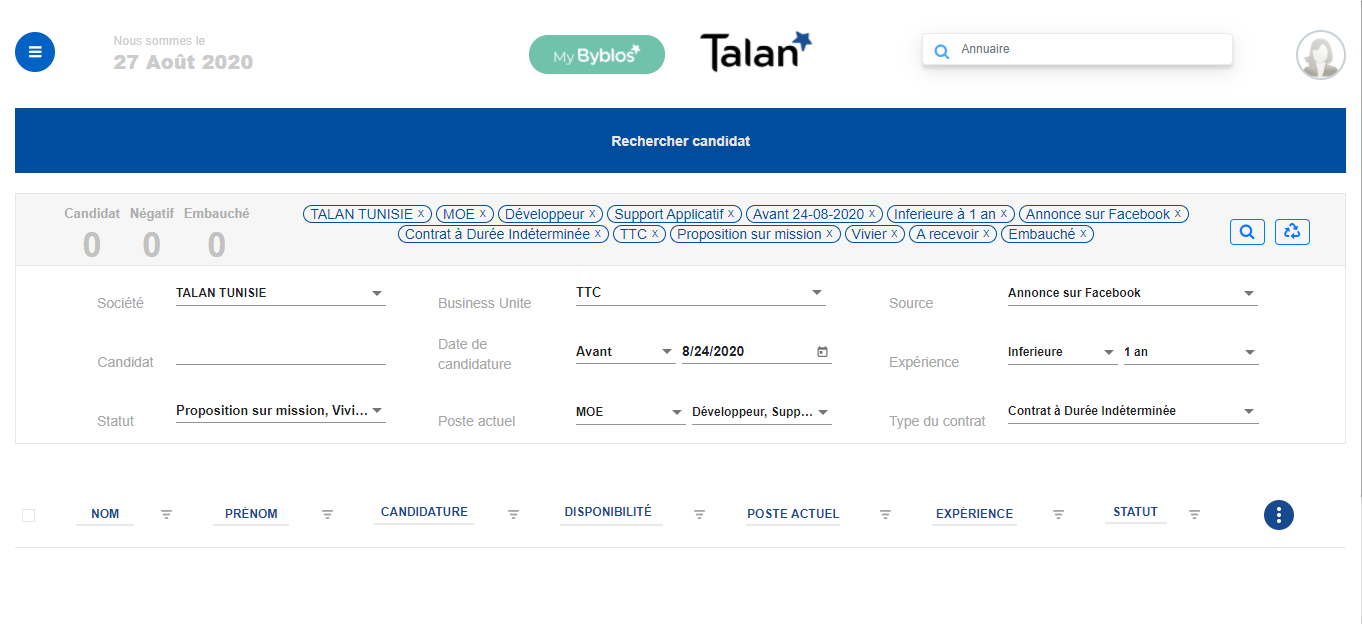
\includegraphics[scale=0.5]{img/capture recherche candidat.PNG}
     \caption{Interface de la recherche d'un candidat}
     \label{fig:capture_recherche}
 \end{figure}
 %%%%%%%%%%%%%%%%%%%%%%%%%%%%%%%%%%%%%%%%%%%%%%%%
 \subsection{Interface du résultat de la recherche}
 Cette interface, représentée dans la Figure \ref{fig:capture_resultat_recherche}, comporte une partie qui contient le nombre total de candidats répondant aux critères de la recherche effectuée, le nombre  de candidats ayant un statut "\textbf{Négatif}" et le nombre  de candidats ayant un statut "\textbf{Embauché}". Elle comporte aussi un tableau détaillant le résultat de la recherche, ainsi qu'un bouton permettant le téléchargement d'un fichier excel qui contient les candidats sélectionnés. 
 \begin{figure}[H]
     \centering
     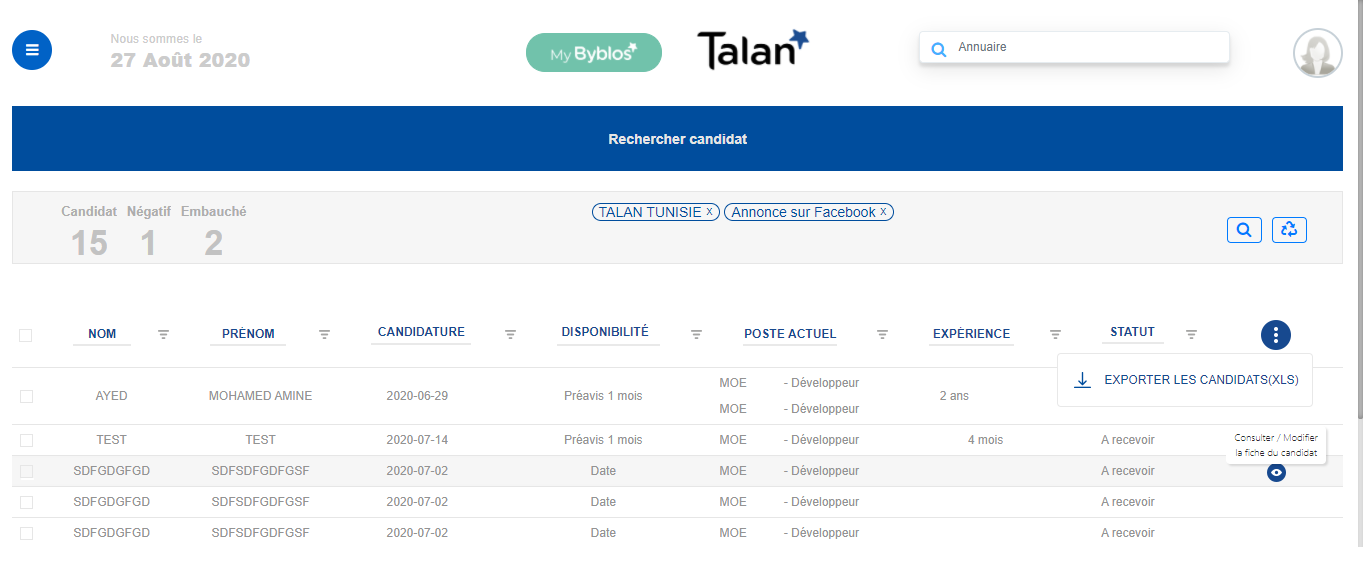
\includegraphics[scale=0.5]{img/capture resultat recherche.png}
     \caption{Interface du résultat de la recherche}
     \label{fig:capture_resultat_recherche}
 \end{figure}
 %%%%%%%%%%%%%%%%%%%%%%%%%%%%%%%%%%%%%%%%%%%%%%%%
 \subsection{Interface du fichier excel contenant le résultat de la recherche}
 Cette interface, représentée dans la Figure \ref{fig:capture_fichier_excel}, comporte le fichier excel téléchargé précédemment et qui contient les différentes informations concernant les candidats sélectionnés.  
 \begin{figure}[H]
     \centering
     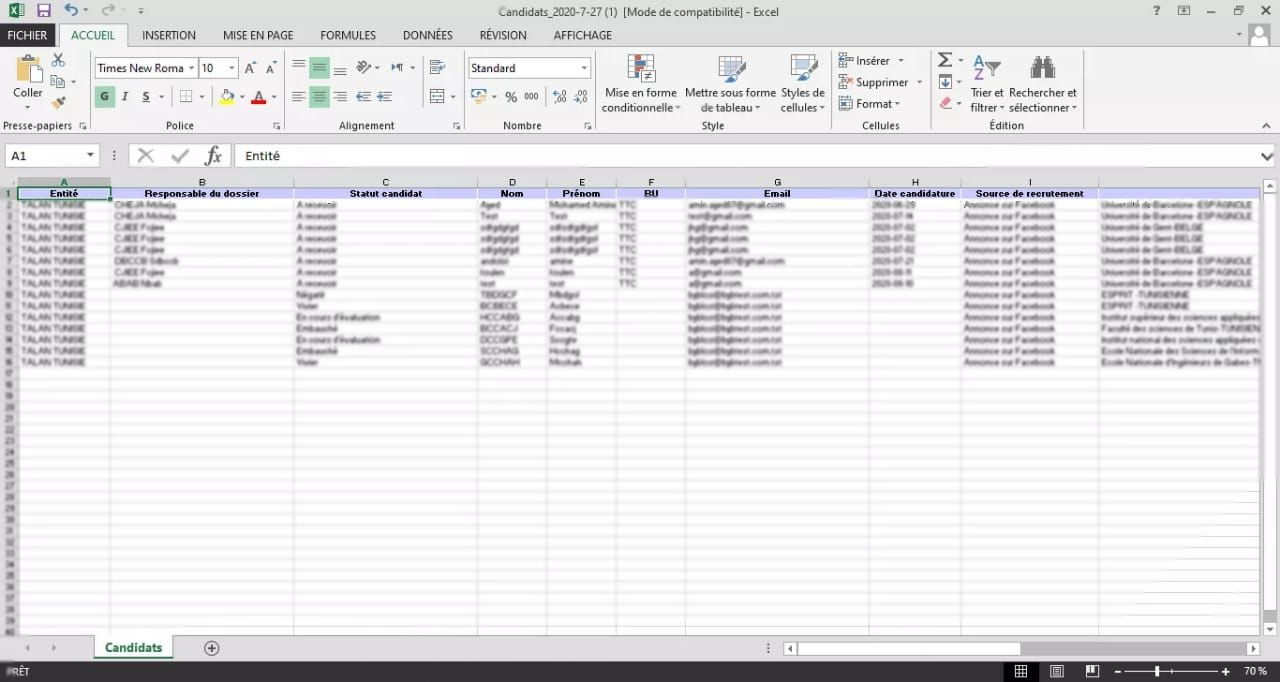
\includegraphics[scale=0.45,width=\textwidth]{img/WhatsApp Image 2020-08-27 at 17.09.20.jpeg}
     \caption{Interface du fichier excel contenant le résultat de recherche}
     \label{fig:capture_fichier_excel}
 \end{figure}
 %%%%%%%%%%%%%%%%%%%%%%%%%%%%%%%%%%%%%%%%%%%%%%%%
 \subsection{Interface de la planification d'un entretien}
 Cette interface, représentée dans la Figure \ref{fig:capture_planifier_entretien}, contient le formulaire utilisé pour planifier un nouvel entretien.
 \begin{figure}[H]
     \centering
     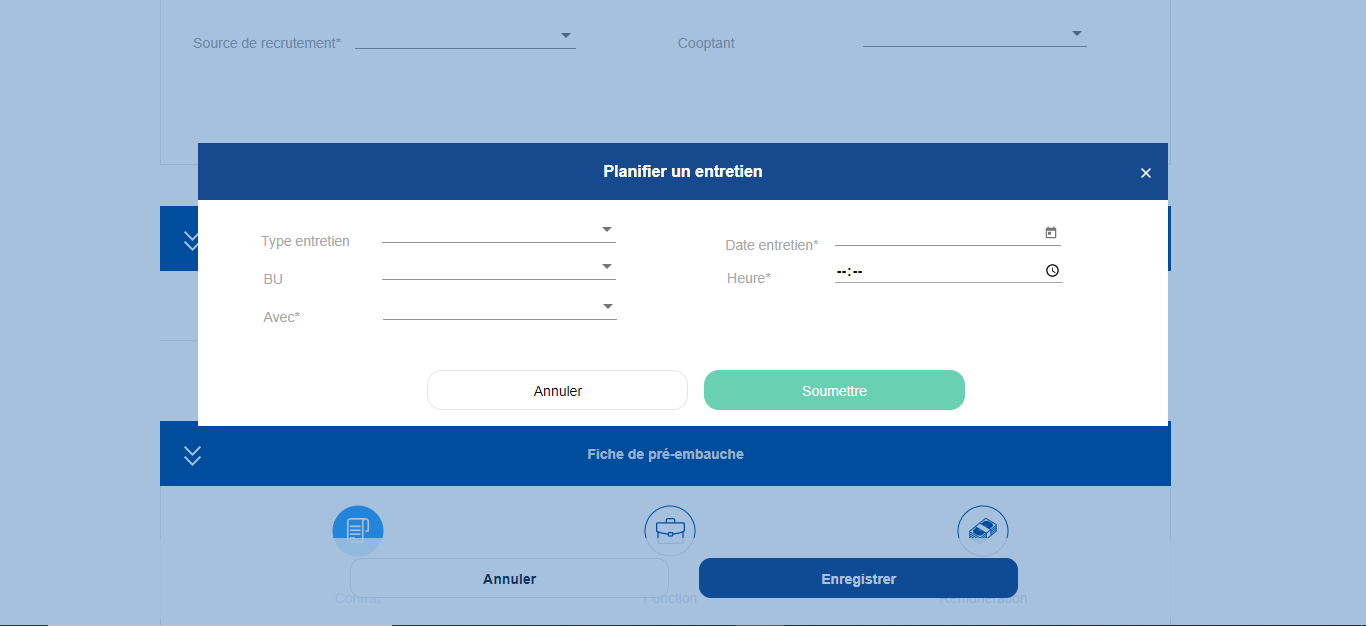
\includegraphics[scale=0.5]{img/capture planifier entretien.PNG}
     \caption{Interface de la planification d'un entretien}
     \label{fig:capture_planifier_entretien}
 \end{figure}
%%%%%%%%%%%%%%%%%%%%%%%%%%%%%%%%%%%%%%%%%%%%%%%%%
\subsection{Interface contenant l'e-mail de validation de l'entretien}
Cette interface, représentée dans la Figure \ref{fig:capture_email_validation}, contient l'e-mail envoyé au recruteur après la planification de l'entretien par le back-office, pour qu'il soit accepté ou refusé.
\begin{figure}[H]
     \centering
     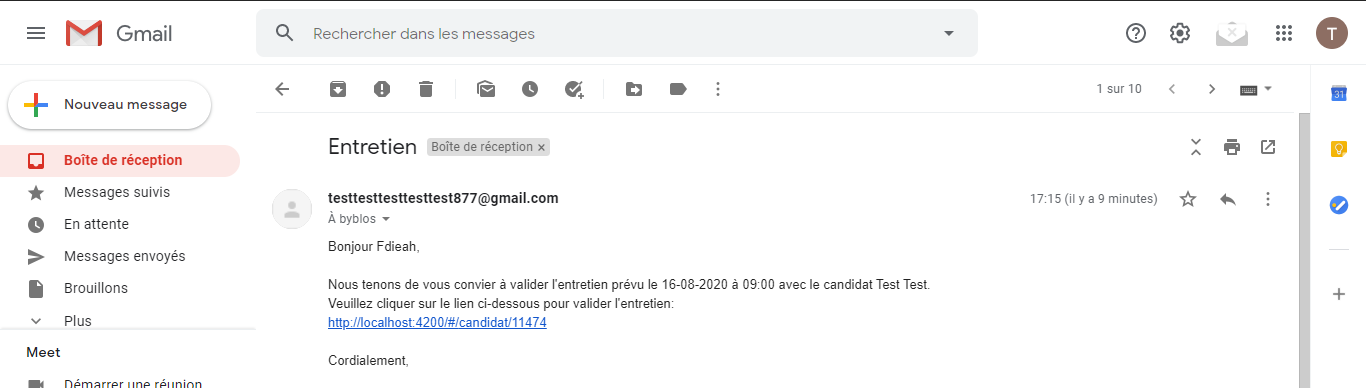
\includegraphics[scale=0.5]{img/capture mail de validation.PNG}
     \caption{Interface contenant l'e-mail de validation de l'entretien}
     \label{fig:capture_email_validation}
 \end{figure}
 %%%%%%%%%%%%%%%%%%%%%%%%%%%%%%%%%%%%%%%%%%%%%%%%
 \subsection{Interface contenant l'e-mail du rejet de l'entretien }
 Si le recruteur rejette l'entretien, un e-mail sera envoyé au back-office pour lui notifier ce refus. Cette interface est représentée dans la Figure \ref{fig:capture_email_rejet}.
 \begin{figure}[H]
     \centering
     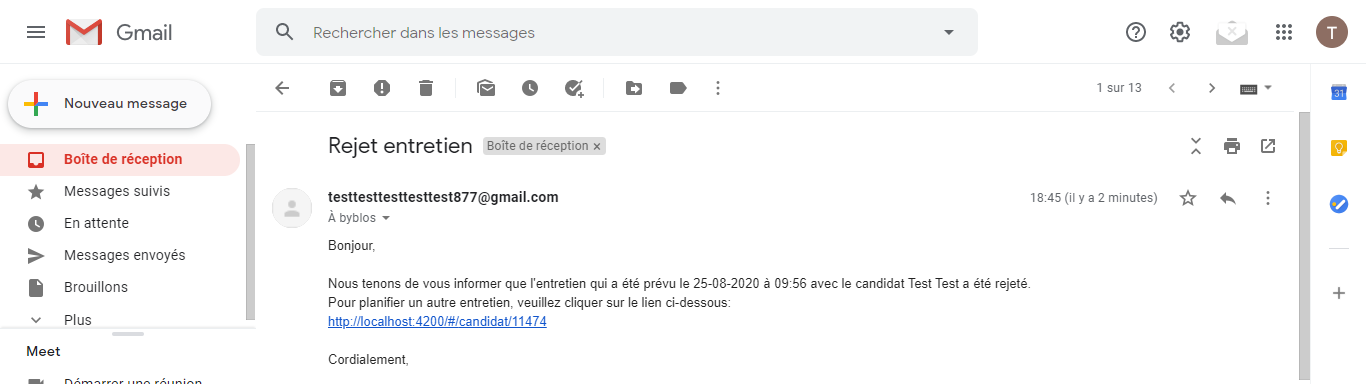
\includegraphics[scale=0.5]{img/capture mail rejet entretien.PNG}
     \caption{Interface contenant l'e-mail du rejet de l'entretien}
     \label{fig:capture_email_rejet}
 \end{figure}
 %%%%%%%%%%%%%%%%%%%%%%%%%%%%%%%%%%%%%%%%%%%%%%%%
\subsection{Interface contenant les différents statuts des entretiens}
Un entretien peut avoir l'un des statuts suivants :
\begin{itemize}
    \item "\textbf{Accepté}" : représenté sous forme d'une icône verte.
    \item "\textbf{Rejeté}" : représenté sous forme d'une icône rouge.
    \item "\textbf{En attente}" : représenté sous forme d'une icône bleue.
\end{itemize}
Cette interface est représentée dans la Figure \ref{fig:capture_liste_entretien}.
\begin{figure}[H]
     \centering
     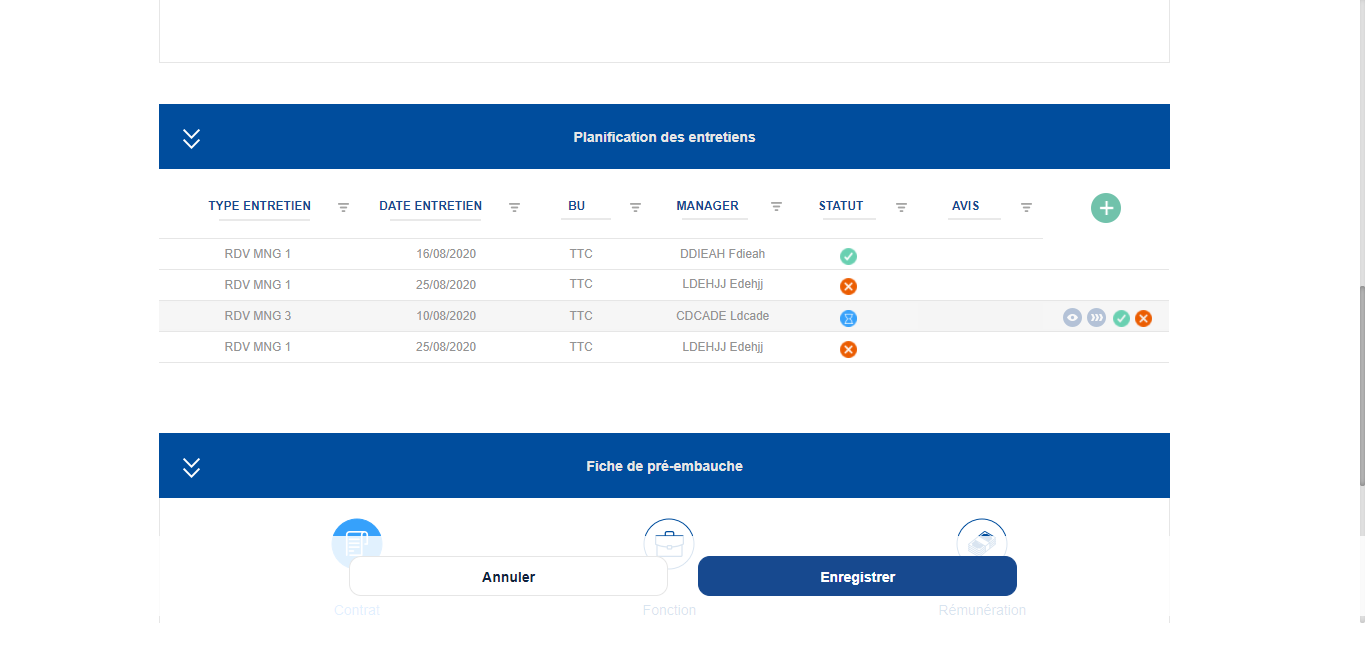
\includegraphics[scale=0.5]{img/cpature liste entretien.png}
     \caption{Interface contenant les différents statuts des entretiens}
     \label{fig:capture_liste_entretien}
 \end{figure}
%%%%%%%%%%%%%%%%%%%%%%%%%%%%%%%%%%%%%%%%%%%%%%%%%
\subsection{Interface de la consultation du Workflow d'un entretien en attente}
Cette interface, montrée dans la Figure \ref{fig:capture_entretien_en_attente}, représente le Workflow d'un entretien qui est en attente de validation par le recruteur.
\begin{figure}[H]
     \centering
     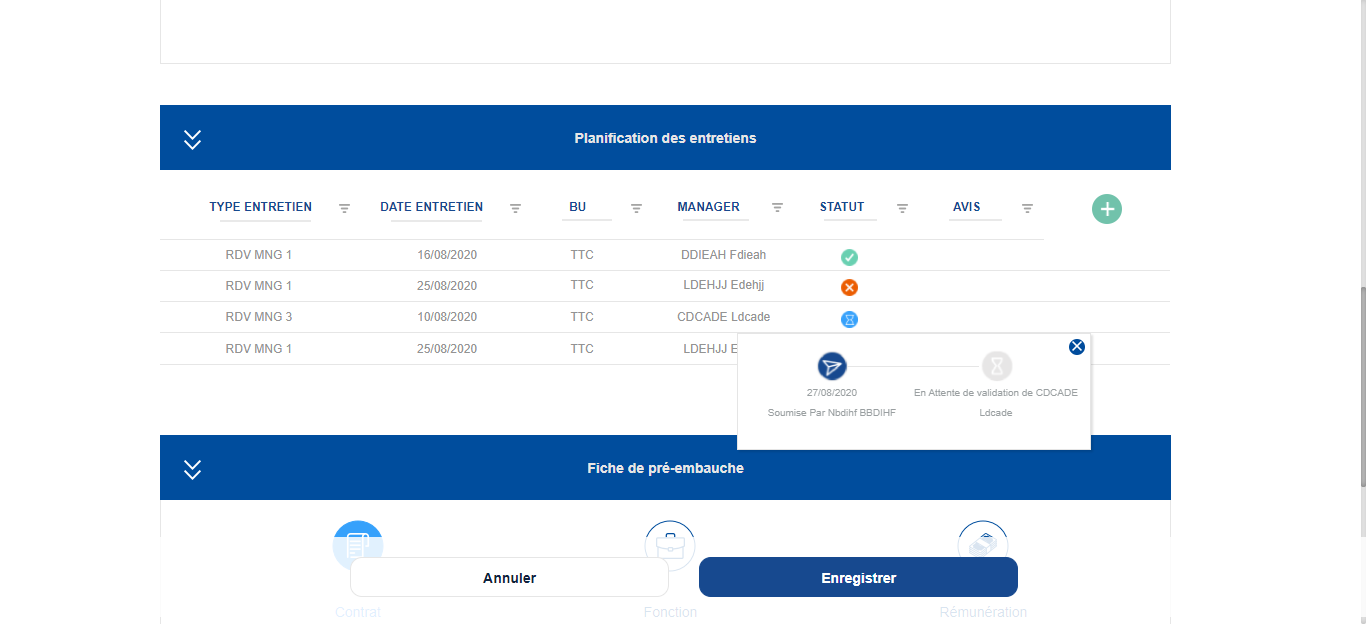
\includegraphics[scale=0.5]{img/capture entretien statut en attente.png}
     \caption{Interface de la consultation du Workflow d'un entretien en attente de validation}
     \label{fig:capture_entretien_en_attente}
 \end{figure}
 %%%%%%%%%%%%%%%%%%%%%%%%%%%%%%%%%%%%%%%%%%%%%%%%
\subsection{Interface de la consultation du Workflow d'un entretien accepté}
Cette interface, représentée dans la Figure  \ref{fig:capture_entretien_accepte}, montre le Workflow d'un entretien accepté.
\begin{figure}[H]
     \centering
     \includegraphics[scale=0.5]{img/capture entretien statut accepté.PNG}
     \caption{Interface de la consultation du Workflow d'un entretien accepté}
     \label{fig:capture_entretien_accepte}
 \end{figure}
 %%%%%%%%%%%%%%%%%%%%%%%%%%%%%%%%%%%%%%%%%%%%%%%%
\subsection{Interface de la consultation du Workflow d'un entretien rejeté}
Cette interface, représentée dans la Figure  \ref{fig:capture_entretien_rejeté}, montre le Workflow d'un entretien rejeté.
\begin{figure}[H]
     \centering
     \includegraphics[scale=0.5]{img/capture entretien statut refusé.PNG}
     \caption{Interface de la consultation du Workflow d'un entretien rejeté}
     \label{fig:capture_entretien_rejeté}
 \end{figure}
%%%%%%%%%%%%%%%%%%%%%%%%%%%%%%%%%%%%%%%%%%%%%%%%%
\section*{Conclusion}
La phase de réalisation est l’étape la plus exigeante en termes d'efforts et de temps. Elle nous a permis de concrétiser et d’approfondir nos connaissances académiques grâce à l’opportunité qui nous a été offerte pour la réalisation d’un projet informatique réel au sein
d’une grande entreprise. Ce chapitre constitue en fait l’aboutissement des phases précédentes. 

        \clearpage
        
        \chapter*{Conclusion générale}
\addcontentsline{toc}{chapter}{Conclusion générale}
\markboth{Conclusion générale}{}
Adopter l'approche des micro-services n'est pas un sujet prospectif, mais une réalité pour les entreprises, d'autant plus que des géants du web comme Netflix et Amazon le trouvent efficace et fiable. En effet, les entreprises devraient accorder dorénavant une grande importance au choix de l'architecture de leur système en vue d'améliorer la performance de leurs activités.\\ \\
Le projet de refonte architecturale de l'ERP "BYBLOS" réalisé par \textbf{Talan Tunisie}, particulièrement le module de gestion des candidats, est un pas en avant vers une agilité de bout en bout. L'objectif final, n'est qu'une pure volonté stratégique, vise à faire évoluer l'organisation de l'entreprise, mais aussi à lui apporter de nouveaux projets plus robustes et plus efficaces.\\ \\
Ainsi, \textbf{Talan Tunisie} a jugé utile d'opter pour l'architecture microservices de son ERP qui permet de pallier à certaines insuffisances de l'architecture monolithique, notamment la lourdeur de la maintenance et l'affectation du système par la défaillance d'une seule partie de ce dernier. Quelques modules ont déjà été migrés vers cette architecture (le module d'authentification, le module RH...). Notre travail a consisté à suivre toutes les étapes nécessaires (analyse préalable, conception, réalisation, intégration) pour assurer une telle migration et bénéficier des ses avantages.\\ \\ 
Signalons toutefois que l'intégration du microservice de gestion des candidats dans le service de découverte et dans le Gateway nous a demandé un effort particulier pour trouver le meilleur moyen de réaliser une telle opération qui constitue pour nous une tâche tout à fait nouvelle.\\ \\
Ce travail est certes perfectible. Certaines fonctionnalités pourront être intégrées ultérieurement dans le module de gestion des candidats. Citons en particulier : 
\begin{itemize}
    \item L'intégration d'un système de notification pour prévenir le recruteur de la planification d'un entretien, et informer le back-office de la validation de l'entretien par le recruteur.
    \item L'intégration d'une liste de questions qui peuvent être posées aux candidats par les recruteurs à chaque étapes de l'entretien.
    \item L'intégration d'un module de Machine Learning qui permet d'analyser les réponses des candidats. 
\end{itemize}
 



        \clearpage
        
		% the command `\nocite{*}` is mandatory to avoid the “no \citation commands” error
        % https://tex.stackexchange.com/questions/18045/problem-with-compiling-bibtex-no-citation-commands-error
        %\nocite{*}
        \printbibliography[heading=bibintoc]
        
        \chapter*{Nétographie}
\addcontentsline{toc}{chapter}{Nétographie}
\markboth{Nétographie}{}
\stepcounter{chapter}
\addtocontents{lot}{\vspace{3.8mm}}
\addtocontents{lof}{\vspace{3.8mm}}

%Mettez vos annexes ici...

%===================== ANNEXE 1 =====================%

\begin{enumerate}[label={[\arabic*]}]
    \item https$:$//tn.talan.com/ (consulté le 21/02/2020)
    \item https$:$//www.occitech.fr/blog/2015/02/les-microservices/ (Consulté le 25/02/2020)
    \item https$:$//blog.codeinsider.fr/architecture-monolith-ou-microservices-laquelle-choisir\\-et-pourquoi/ (Consulté le 15/03/2020)
    \item https$:$//www.ionos.fr/digitalguide/sites-internet/developpement-web/architecture-microservices/ (Consulté le 22/03/2020)
    \item https$:$//openclassrooms.com/fr/courses/4668056-construisez-des-microservices/\\5122300-apprehendez-larchitecture-microservices (Consulté le 12/05/2020)
    \item https$:$//www.redhat.com/fr/topics/microservices/what-are-microservices (Consulté le 26/05/2020)
   \item https$:$//cloud.google.com/solutions/migrating-a-monolithic-app-to-microservices-gke?hl=fr (Consulté le 13/06/2020)
   \item https$:$//juliendubreuil.fr/blog/developpement/de-application-monolithique-aux-architectures\\-microservices-ou-orientees-composants/ (Consulté le 23/06/2020)
\end{enumerate}

   


        \clearpage
        \newpage

        \backmatter
        
%== It's advised to not modify the content of this file ===%
% To set your information, go to global_config.tex file    %
%==========================================================%

\thispagestyle{backcover}
\newgeometry{bottom=25mm,left=15mm,top=20mm,right=15mm}

\begin{changemargin}{3mm}{0cm}
    \begin{minipage}[c]{0.96\columnwidth}
        
        
        
        {\LARGE\textbf{Résumé}}
        \vskip1mm
            \begingroup
                \large
                \@frenchAbstract
            \endgroup
        \vskip1mm
        {\textbf{Mots clés : }
            \begingroup
                \@frenchAbstractKeywords
            \endgroup
        }
        
        {\ifthenelse{\boolean{wantToTypeCompanyAddress}}
        {% IF TRUE
            \vskip5mm
        }{\vskip8mm}}
        
        {\LARGE\textbf{Abstract}}
        \vskip1mm
            \begingroup
                \large
                \@englishAbstract
            \endgroup
        \vskip1mm
        {\textbf{Keywords : }
            \begingroup
                \@englishAbstractKeywords
            \endgroup
        }
    \end{minipage}
    
\end{changemargin}
        
\end{document}